## https://rstudio-pubs-static.s3.amazonaws.com/228019_f0c39e05758a4a51b435b19dbd321c23.html#13_histogram_plots


\section{Plot Two Variables - X \& Y: Both Continuous or Discrete}
\subsection{Scatter plots: Continuous X and Y}
\begin{itemize}
  \item geom\_pint()
  \item geom\_smooth()
  \item geom\_quantile()
  \item geom\_rug()
  \item geom\_jitter()
  \item geom\_text()
\end{itemize}
geom\_point\newline
\textbf{alpha, color, fill, shape, size}

\begin{lstlisting}[language=html]
# Data format
> mtcars
                     mpg cyl  disp  hp drat    wt  qsec vs am gear carb
Mazda RX4           21.0   6 160.0 110 3.90 2.620 16.46  0  1    4    4
Mazda RX4 Wag       21.0   6 160.0 110 3.90 2.875 17.02  0  1    4    4
Datsun 710          22.8   4 108.0  93 3.85 2.320 18.61  1  1    4    1
Hornet 4 Drive      21.4   6 258.0 110 3.08 3.215 19.44  1  0    3    1
Hornet Sportabout   18.7   8 360.0 175 3.15 3.440 17.02  0  0    3    2
Valiant             18.1   6 225.0 105 2.76 3.460 20.22  1  0    3    1
Duster 360          14.3   8 360.0 245 3.21 3.570 15.84  0  0    3    4
Merc 240D           24.4   4 146.7  62 3.69 3.190 20.00  1  0    4    2
Merc 230            22.8   4 140.8  95 3.92 3.150 22.90  1  0    4    2
Merc 280            19.2   6 167.6 123 3.92 3.440 18.30  1  0    4    4
Merc 280C           17.8   6 167.6 123 3.92 3.440 18.90  1  0    4    4
Merc 450SE          16.4   8 275.8 180 3.07 4.070 17.40  0  0    3    3
Merc 450SL          17.3   8 275.8 180 3.07 3.730 17.60  0  0    3    3
Merc 450SLC         15.2   8 275.8 180 3.07 3.780 18.00  0  0    3    3
Cadillac Fleetwood  10.4   8 472.0 205 2.93 5.250 17.98  0  0    3    4
Lincoln Continental 10.4   8 460.0 215 3.00 5.424 17.82  0  0    3    4
Chrysler Imperial   14.7   8 440.0 230 3.23 5.345 17.42  0  0    3    4
Fiat 128            32.4   4  78.7  66 4.08 2.200 19.47  1  1    4    1
Honda Civic         30.4   4  75.7  52 4.93 1.615 18.52  1  1    4    2
Toyota Corolla      33.9   4  71.1  65 4.22 1.835 19.90  1  1    4    1
Toyota Corona       21.5   4 120.1  97 3.70 2.465 20.01  1  0    3    1
Dodge Challenger    15.5   8 318.0 150 2.76 3.520 16.87  0  0    3    2
AMC Javelin         15.2   8 304.0 150 3.15 3.435 17.30  0  0    3    2
Camaro Z28          13.3   8 350.0 245 3.73 3.840 15.41  0  0    3    4
Pontiac Firebird    19.2   8 400.0 175 3.08 3.845 17.05  0  0    3    2
Fiat X1-9           27.3   4  79.0  66 4.08 1.935 18.90  1  1    4    1
Porsche 914-2       26.0   4 120.3  91 4.43 2.140 16.70  0  1    5    2
Lotus Europa        30.4   4  95.1 113 3.77 1.513 16.90  1  1    5    2
Ford Pantera L      15.8   8 351.0 264 4.22 3.170 14.50  0  1    5    4
Ferrari Dino        19.7   6 145.0 175 3.62 2.770 15.50  0  1    5    6
Maserati Bora       15.0   8 301.0 335 3.54 3.570 14.60  0  1    5    8
Volvo 142E          21.4   4 121.0 109 4.11 2.780 18.60  1  1    4    2
\end{lstlisting}
\begin{lstlisting}[language=html]
> b <- ggplot(mtcars, aes(x = wt, y= mpg))
# x weight
# y miles/gallon
#Basic scatter plots
> b + geom_point(color = "#00AFBB")
\end{lstlisting}

\begin{figure}[H]\begin{center}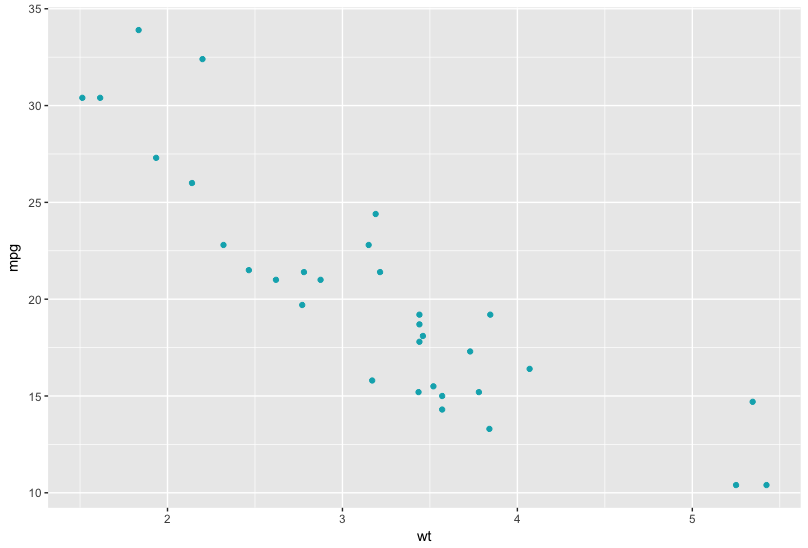
\includegraphics[scale=1 ]{ilu/bg35.png}\end{center}\end{figure}
\begin{lstlisting}[language=html]
# Change the point size, and shape
> b + geom_point(color = "#00AFBB", size = 2, shape = 23)
\end{lstlisting}
\begin{figure}[H]\begin{center}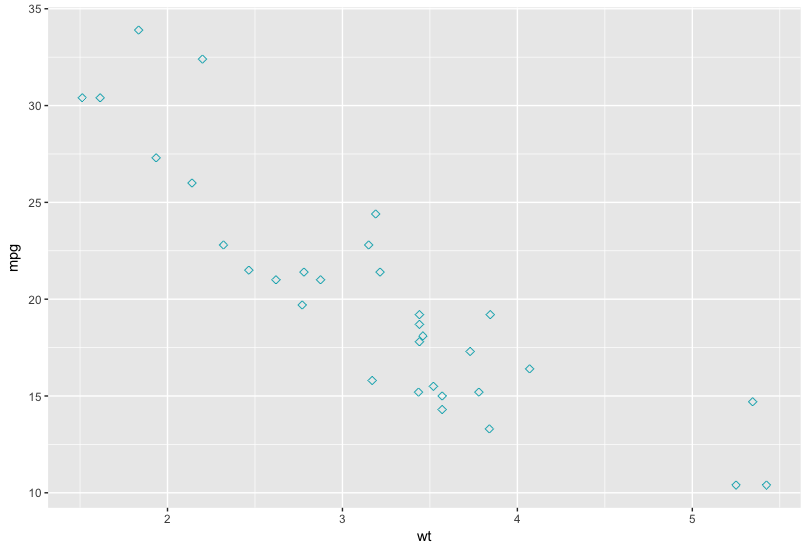
\includegraphics[scale=1 ]{ilu/bg36.png}\end{center}\end{figure}
\begin{lstlisting}[language=html]
# Control point size by continuous variable values
# qsec 1/4 mile time
> b + geom_point(aes(size = qsec), color = "#00AFBB")
\end{lstlisting}
\begin{figure}[H]\begin{center}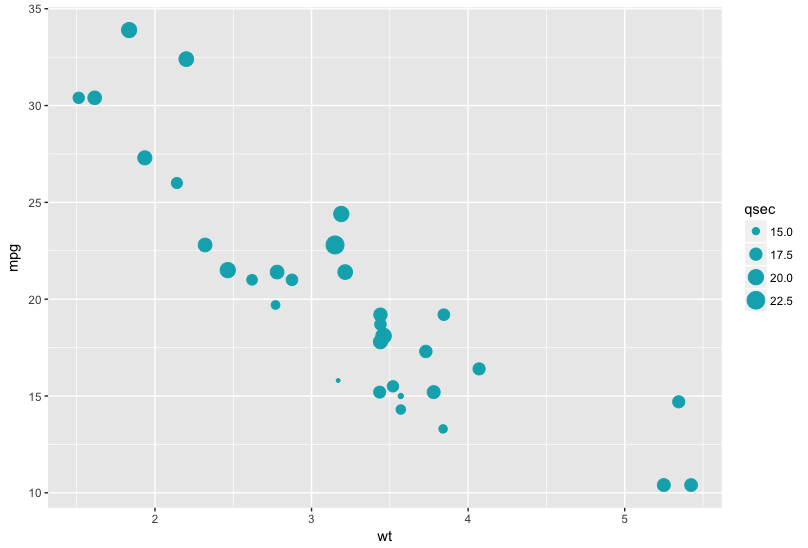
\includegraphics[scale=1 ]{ilu/bg37.png}\end{center}\end{figure}
\begin{lstlisting}[language=html]
# Label text
> b + geom_point() + geom_text(label = rownames(mtcars), nudge_y = 0.8)
\end{lstlisting}
\begin{figure}[H]\begin{center}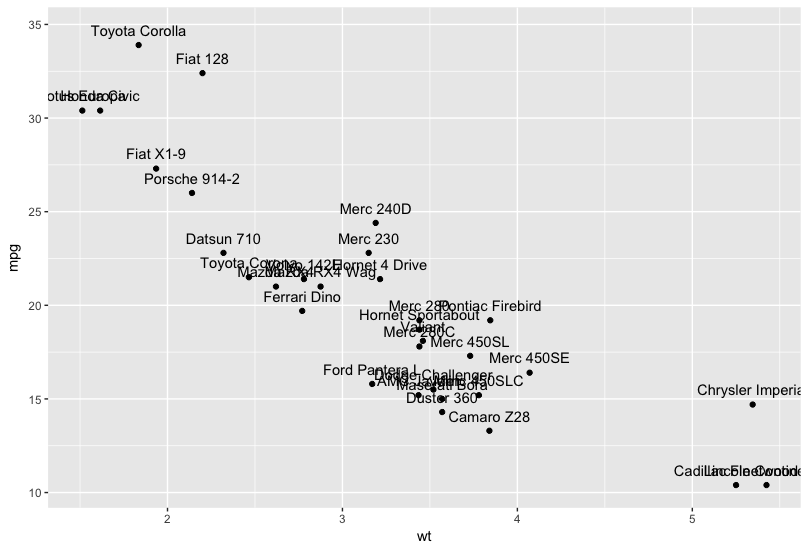
\includegraphics[scale=1 ]{ilu/bg38.png}\end{center}\end{figure}
\begin{lstlisting}[language=html]
# Change shape, color, size automatically
# Change point shape by the level of cyl
> b + geom_point(aes(shape = factor(cyl)))
\end{lstlisting}
\begin{figure}[H]\begin{center}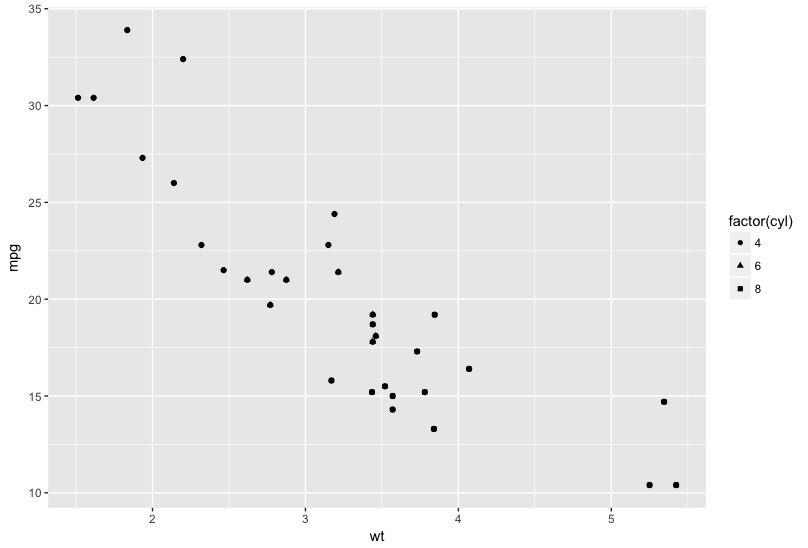
\includegraphics[scale=1 ]{ilu/bg39.png}\end{center}\end{figure}
\begin{lstlisting}[language=html]
# Change point shape and colors
> b + geom_point(aes(color = cyl, shape=factor(cyl)))
\end{lstlisting}
\begin{figure}[H]\begin{center}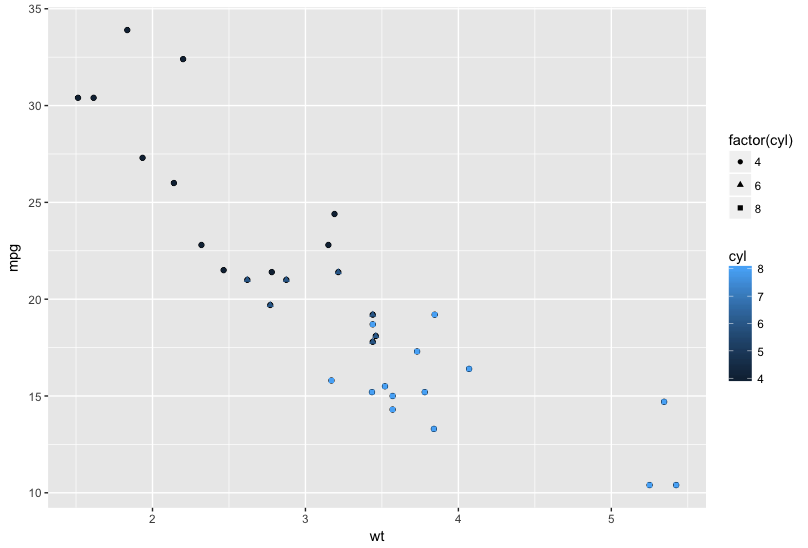
\includegraphics[scale=1 ]{ilu/bg40.png}\end{center}\end{figure}
\begin{lstlisting}[language=html]
# Change shape, color, size manually
# Change the point sizes manually
> b + geom_point(aes(color = cyl, shape=factor(cyl), size = factor(cyl))) + scale_size_manual(values = c(2,3,4))
\end{lstlisting}
\begin{figure}[H]\begin{center}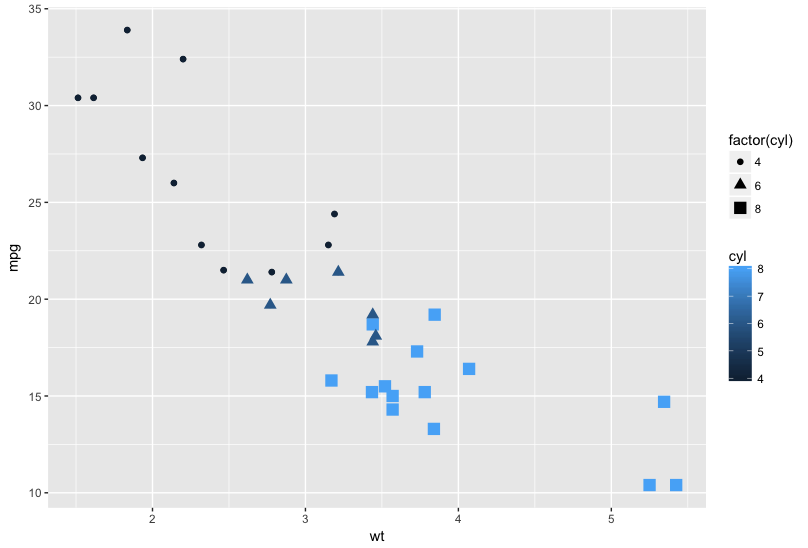
\includegraphics[scale=1 ]{ilu/bg41.png}\end{center}\end{figure}
\begin{lstlisting}[language=html]
# Change the point shapes and colors manually
> b + geom_point(aes(color = cyl, shape = cyl)) + scale_shape_manual(values = c(3,16,17)) + scale_color_manual(values = c('#999999','#E69F00', '#56B4E9'))
Erreur : Continuous value supplied to discrete scale
\end{lstlisting}
\begin{figure}[H]\begin{center}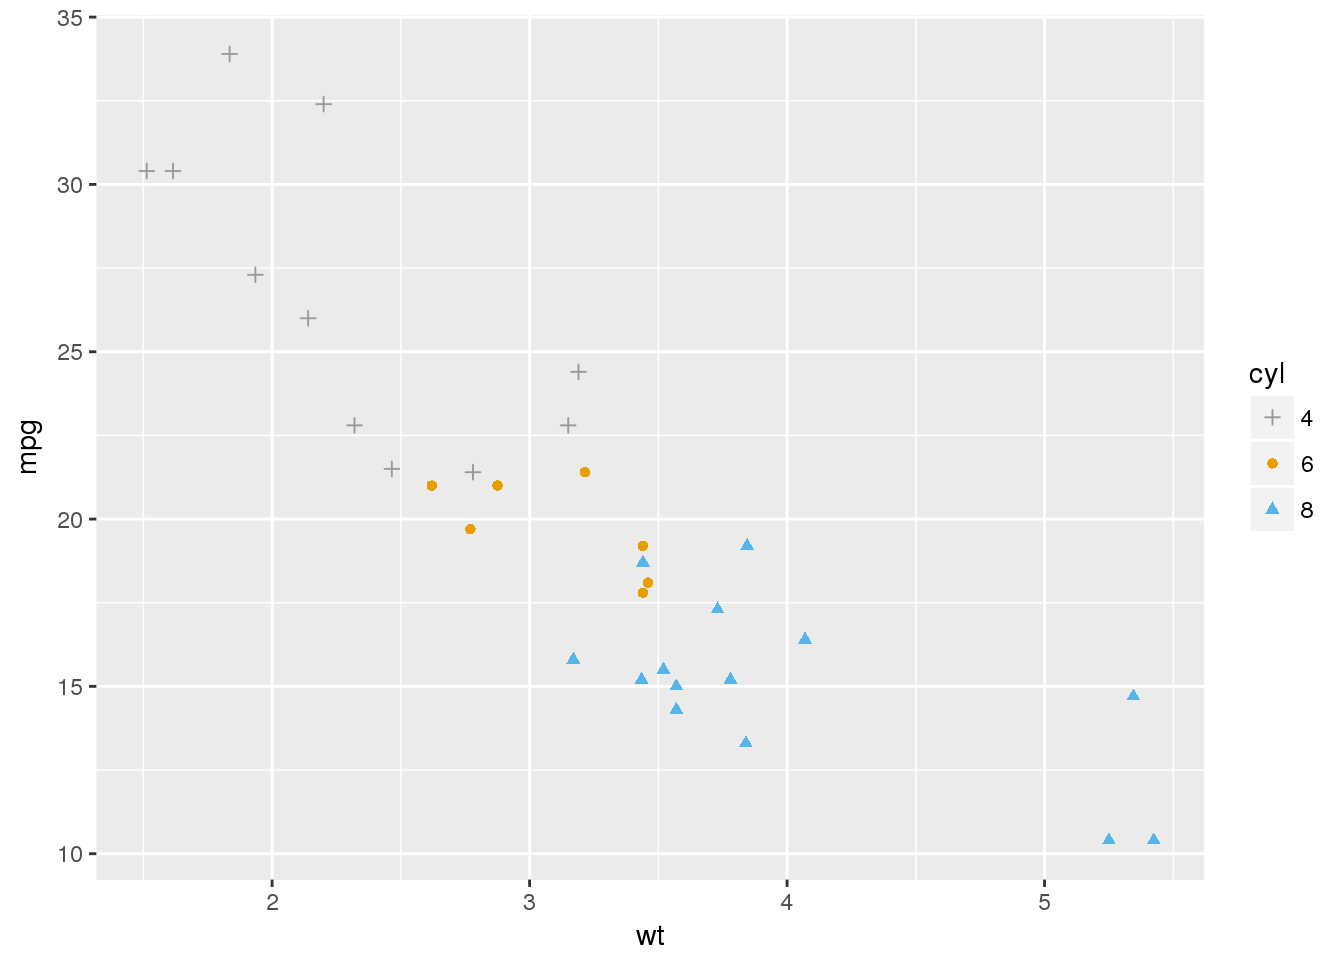
\includegraphics[scale=1 ]{ilu/bg42.png}\end{center}\end{figure}
\begin{lstlisting}[language=html]
# Use brewer color palettes
> b + geom_point(aes(color = cyl, shape = factor(cyl))) + scale_color_brewer(palette = "Dark2") + theme_minimal()
Erreur : Continuous value supplied to discrete scale
\end{lstlisting}
\begin{figure}[H]\begin{center}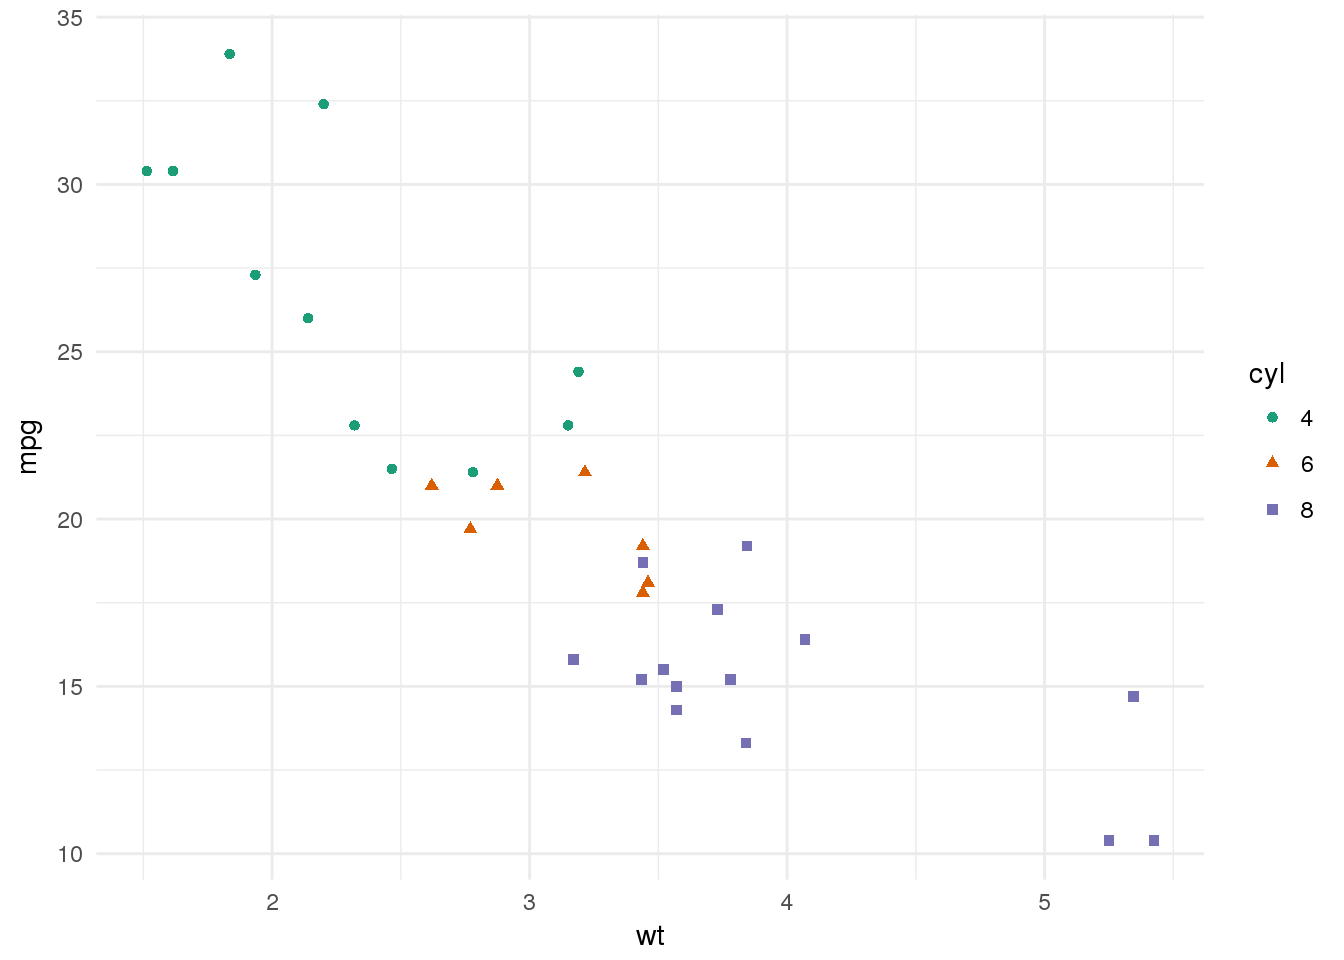
\includegraphics[scale=1 ]{ilu/bg43.png}\end{center}\end{figure}
\begin{lstlisting}[language=html]
# Use grey scale
> b + geom_point(aes(color = cyl, shape = factor(cyl))) + scale_color_grey() + theme_minimal()
Erreur : Continuous value supplied to discrete scale
\end{lstlisting}
\begin{figure}[H]\begin{center}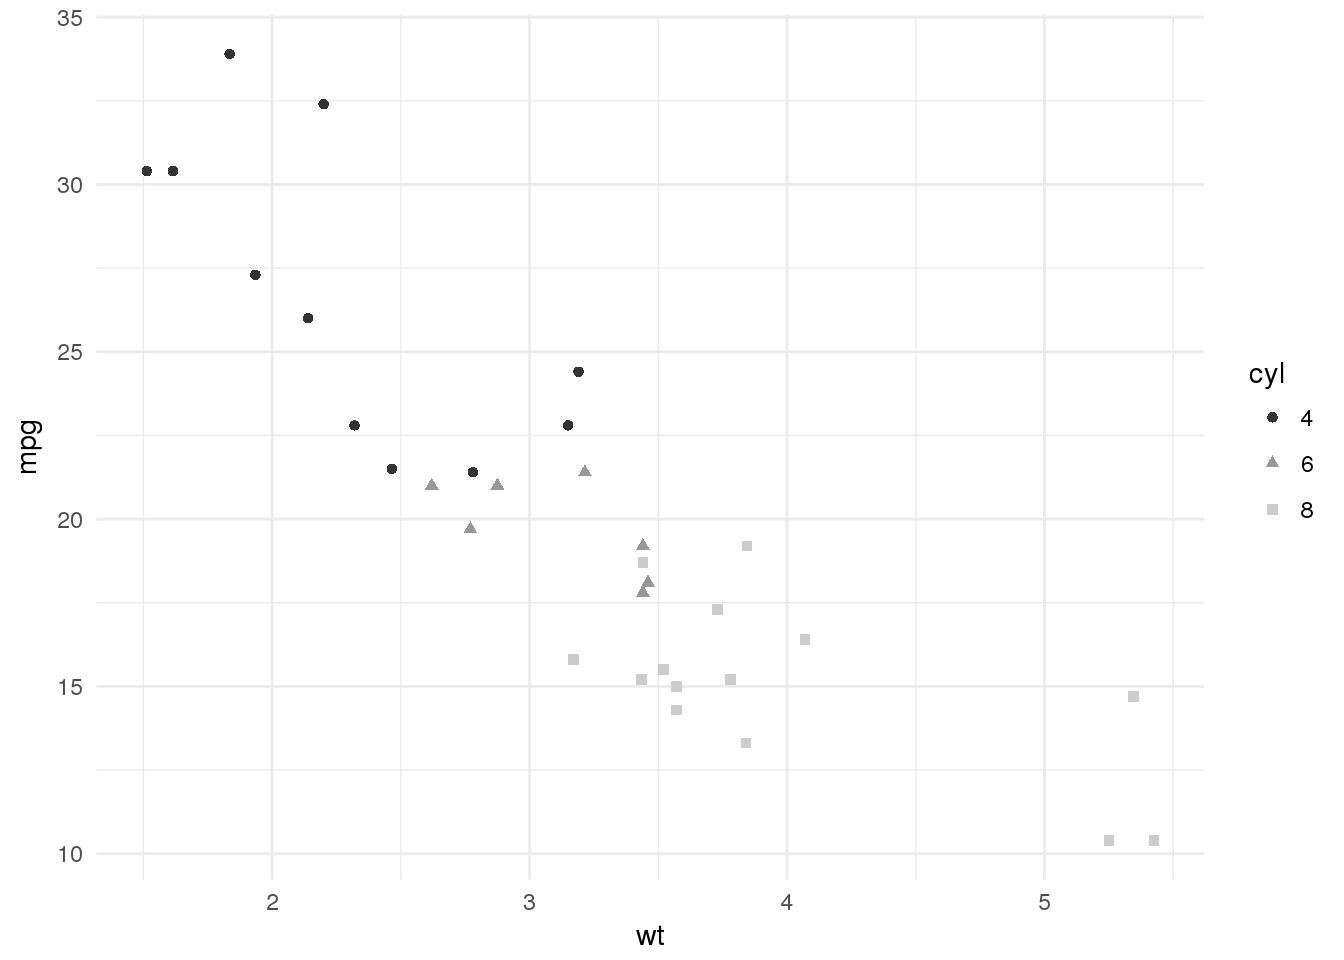
\includegraphics[scale=1 ]{ilu/bg44.png}\end{center}\end{figure}

\textbf{Add regression line or smoothed conditional mean}
\begin{lstlisting}[language=html]
#geom_smooth(), geom_abline()
#alpha, color, fill, shape, linetype, size
#geom_smooth(method = "auto")
#method:loess->local regression, lm-> linear regression

# Add regression line
> b + geom_point() + geom_smooth(method = lm)
\end{lstlisting}
\begin{figure}[H]\begin{center}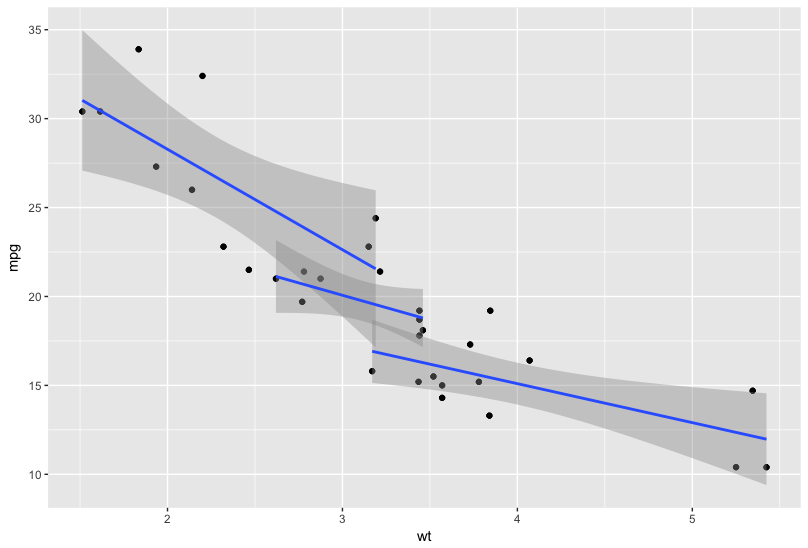
\includegraphics[scale=1 ]{ilu/bg45.png}\end{center}\end{figure}
\begin{lstlisting}[language=html]
# Point + regression line
# Remove the confidence interval
> b + geom_point() + geom_smooth(method = lm, se = FALSE)
\end{lstlisting}
\begin{figure}[H]\begin{center}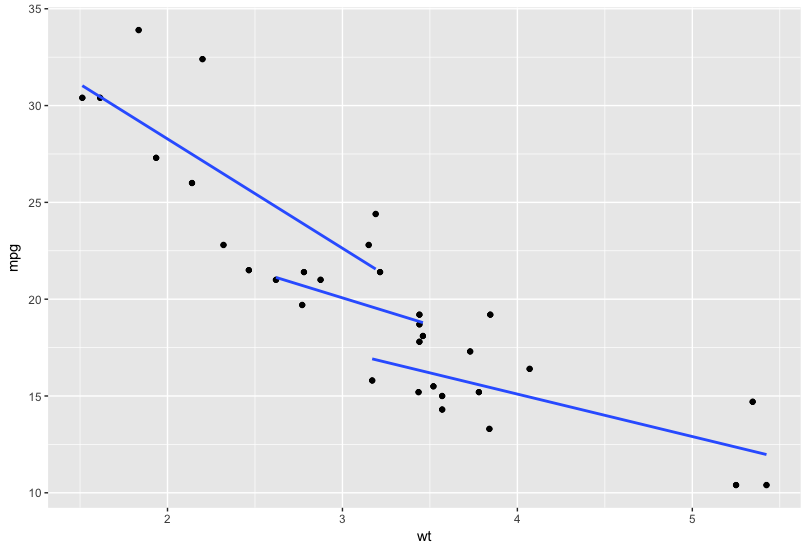
\includegraphics[scale=1 ]{ilu/bg46.png}\end{center}\end{figure}
\begin{lstlisting}[language=html]
# loess method, local regression fitting
> b + geom_point() + geom_smooth()
\end{lstlisting}
\begin{figure}[H]\begin{center}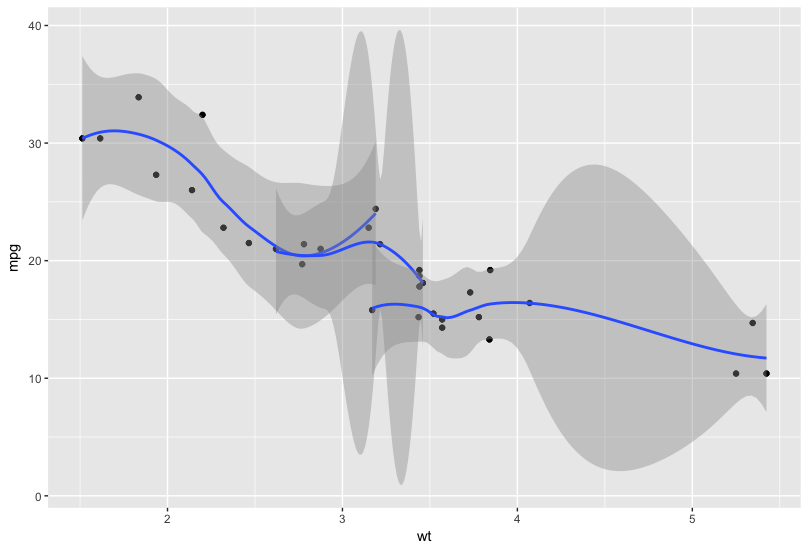
\includegraphics[scale=1 ]{ilu/bg47.png}\end{center}\end{figure}
\begin{lstlisting}[language=html]
# Change the color and shape by groups 
> b + geom_point(aes(color = cyl, shape = factor(cyl))) + geom_smooth(aes(color = cyl, fill = cyl), method = lm)
\end{lstlisting}
\begin{figure}[H]\begin{center}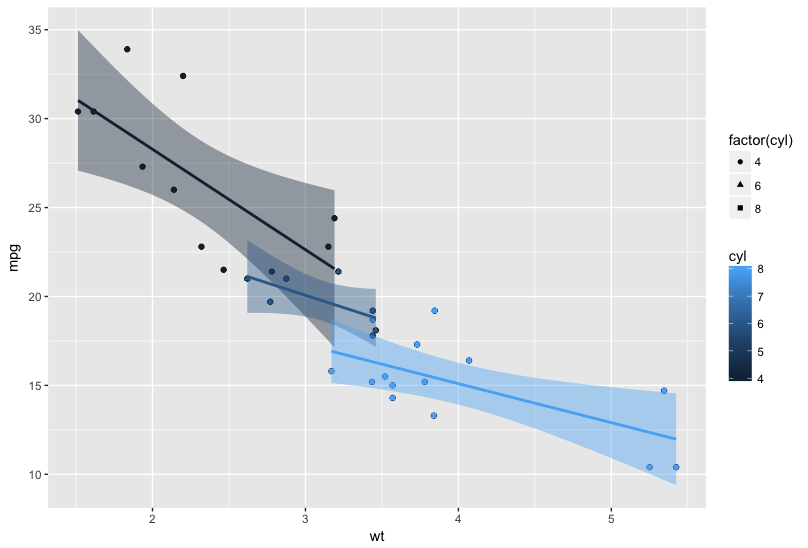
\includegraphics[scale=1 ]{ilu/bg48.png}\end{center}\end{figure}
\begin{lstlisting}[language=html]
# Remove confidence intervals
# Extend the regression lines: fullrage
> b + geom_point(aes(color = cyl, shape = factor(cyl))) + geom_smooth(aes(color = cyl), method = lm, se = FALSE, fullrange = TRUE)
\end{lstlisting}
\begin{figure}[H]\begin{center}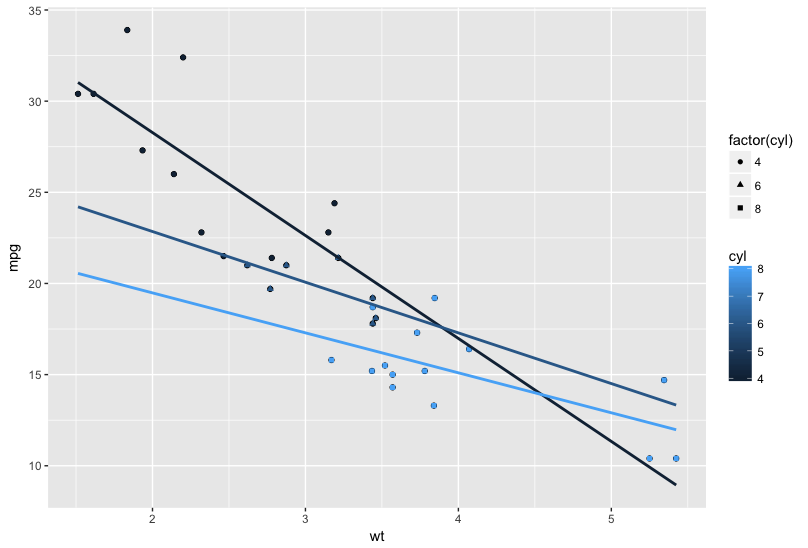
\includegraphics[scale=1 ]{ilu/bg49.png}\end{center}\end{figure}
\begin{lstlisting}[language=html]
# Add marginal rugs to a scatter plot
#geom_rug(sides = "bl")
# sides: a string, "trbl", top, right, bottom, left.
# Add marginal rugs
> b + geom_point() + geom_rug()
\end{lstlisting}
\begin{figure}[H]\begin{center}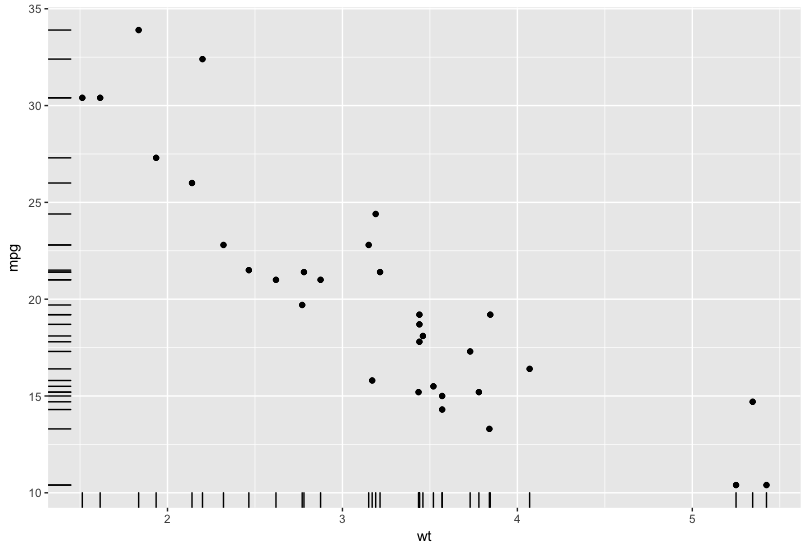
\includegraphics[scale=1 ]{ilu/bg50.png}\end{center}\end{figure}
\begin{lstlisting}[language=html]
# Change the color by group
> b +\end{lstlisting} geom_point(aes(color = cyl)) + geom_rug(aes(color = cyl))

\begin{figure}[H]\begin{center}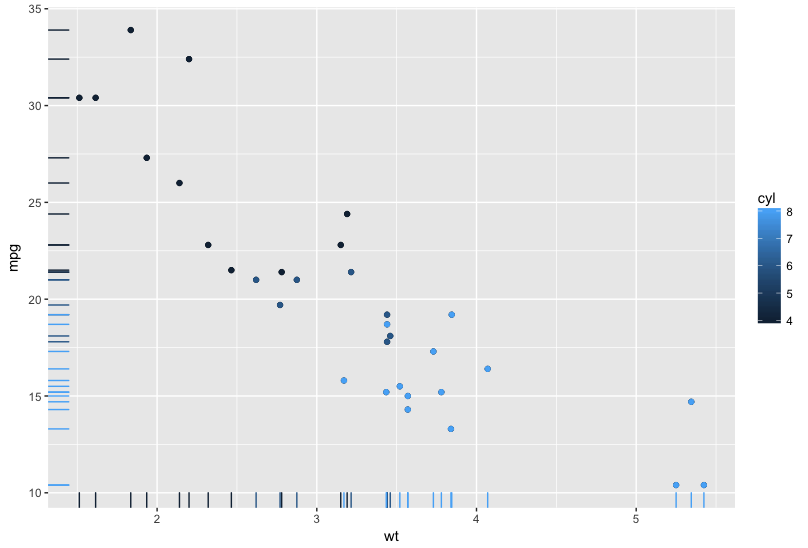
\includegraphics[scale=1 ]{ilu/bg51.png}\end{center}\end{figure}
\begin{lstlisting}[language=html]
# Add marginal rugs using faithful data
> data(faithful)
> faithful <- as_data_frame(faithful)
> faithful
# A tibble: 272 x 2
   eruptions waiting
 *     <dbl>   <dbl>
 1     3.600      79
 2     1.800      54
 3     3.333      74
 4     2.283      62
 5     4.533      85
 6     2.883      55
 7     4.700      88
 8     3.600      85
 9     1.950      51
10     4.350      85
# ... with 262 more rows
\end{lstlisting}
\textcolor{white}{.}\newline
\begin{lstlisting}[language=html]
> ggplot(faithful, aes(x = eruptions, y = waiting)) + geom_point() + geom_rug()
\end{lstlisting}
\begin{figure}[H]\begin{center}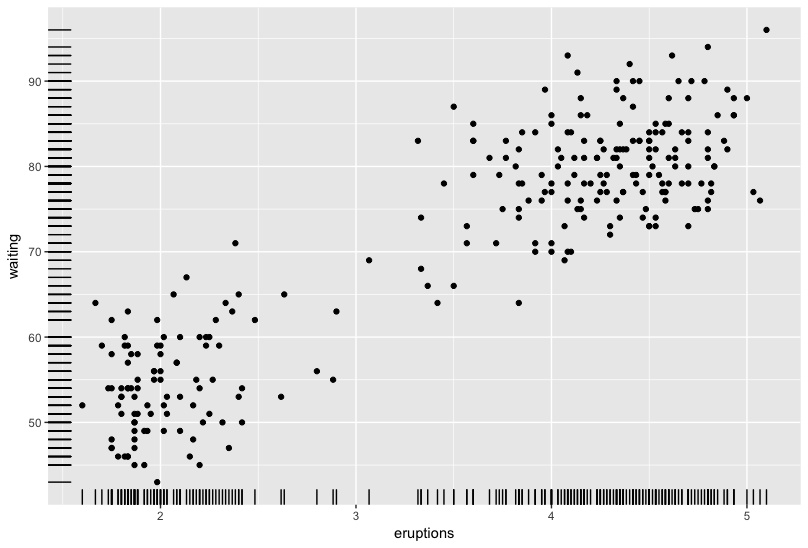
\includegraphics[scale=1 ]{ilu/bg52.png}\end{center}\end{figure}
\begin{lstlisting}[language=html]
# Jitter points to reduce overplotting
# geom_jitter(), position_jitter()
#alpha, color, fill, shape, size

# Use mpg data
> p <- ggplot(mpg, aes(displ, hwy))

# Default sactter plot
> p + geom_point()
\end{lstlisting}
\begin{figure}[H]\begin{center}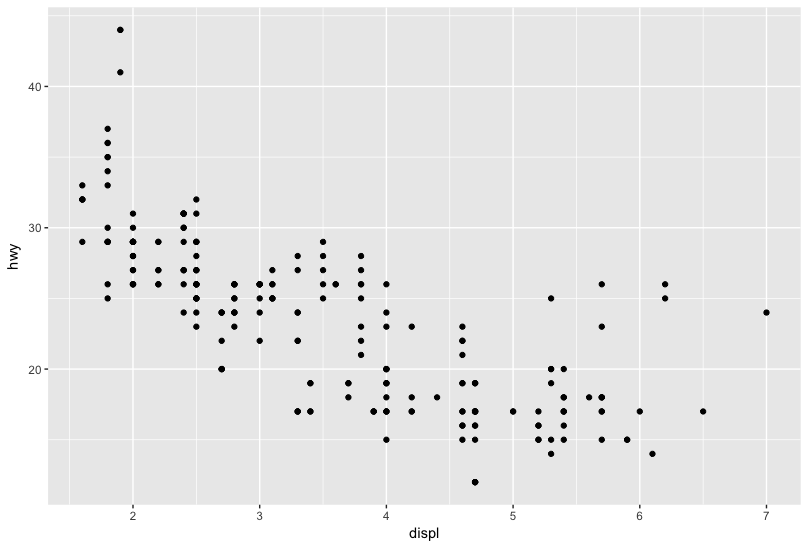
\includegraphics[scale=1 ]{ilu/bg53.png}\end{center}\end{figure}
\begin{lstlisting}[language=html]
# Use jitter to reduce overplotting
> p + geom_jitter(position = position_jitter(width = 0.5, height = 0.5))
\end{lstlisting}
\begin{figure}[H]\begin{center}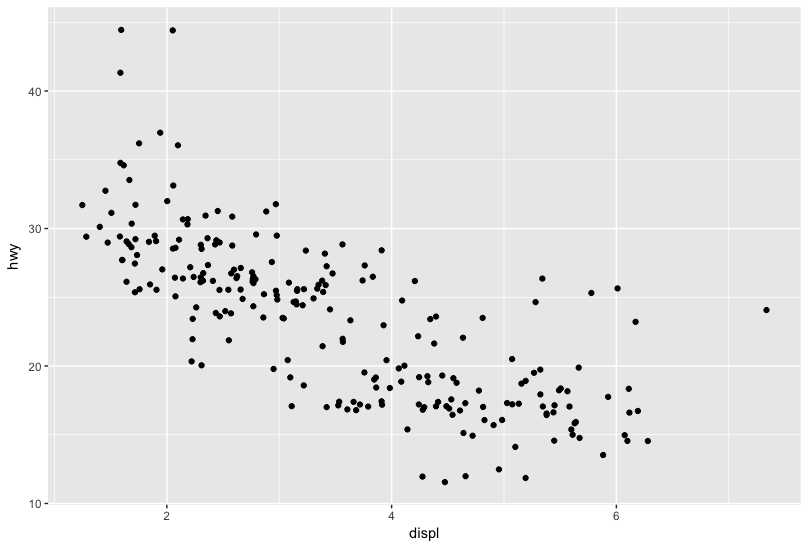
\includegraphics[scale=1 ]{ilu/bg54.png}\end{center}\end{figure}
\begin{lstlisting}[language=html]
> select(mpg, displ, hwy) %>% arrange(-hwy) %>% filter(displ == 1.9)
# A tibble: 3 x 2
  displ   hwy
  <dbl> <int>
1   1.9    44
2   1.9    44
3   1.9    41
\end{lstlisting}
\textcolor{white}{.}\newline
\begin{lstlisting}[language=html]
##
#Text annotation
#geom_text()
#label, alpha, angle, color, family, fontface, hjust, lineheight, size, vjust

> b + geom_text(aes(label = rownames(mtcars)), size = 3)
\end{lstlisting}
\begin{figure}[H]\begin{center}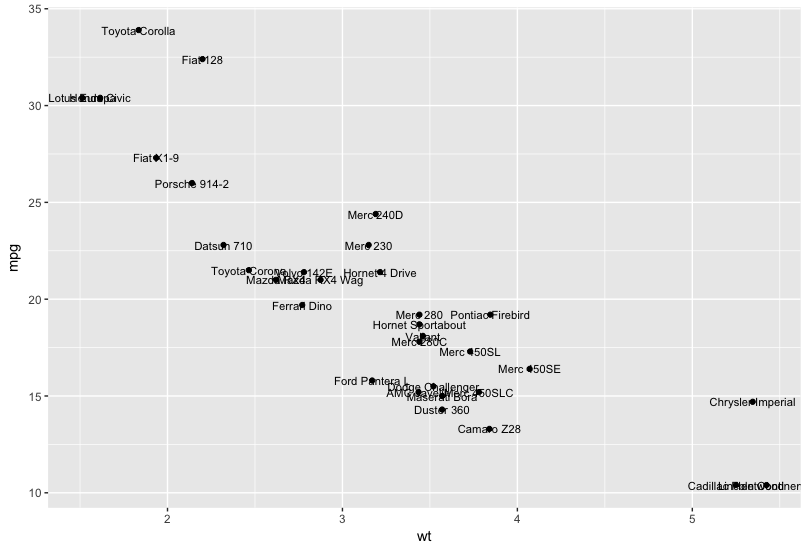
\includegraphics[scale=1 ]{ilu/bg55.png}\end{center}\end{figure}

\subsection{Continuous bivariate distribution}
\begin{itemize}
  \item geom\_bin2d()
  \item geom\_hex()
  \item geom\_density\_2d()
\end{itemize}

\begin{lstlisting}[language=html]
> data("diamonds")
> c <- ggplot(diamonds, aes(carat, price))
# Add heatmap of 2d bin counts
# geom_bin2d produce a scatter plot with rectangular bins.
# stat_bin_2d(), stat_summary_2d()
# max, xmin, ymax, ymin, alpha, color, fill, linetype, size
> c + geom_bin2d()
\end{lstlisting}
\begin{figure}[H]\begin{center}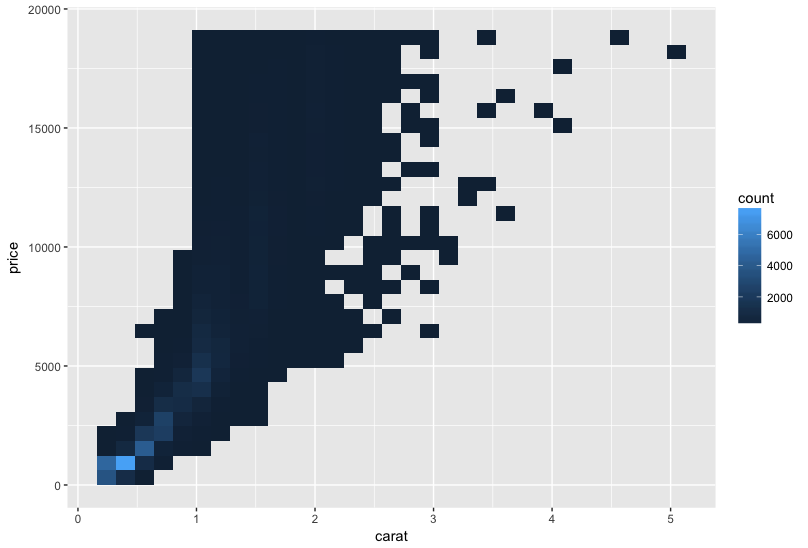
\includegraphics[scale=1 ]{ilu/bg56.png}\end{center}\end{figure}
\begin{lstlisting}[language=html]
# Change the number of bins
> c + geom_bin2d(bins = 15)
\end{lstlisting}
\begin{figure}[H]\begin{center}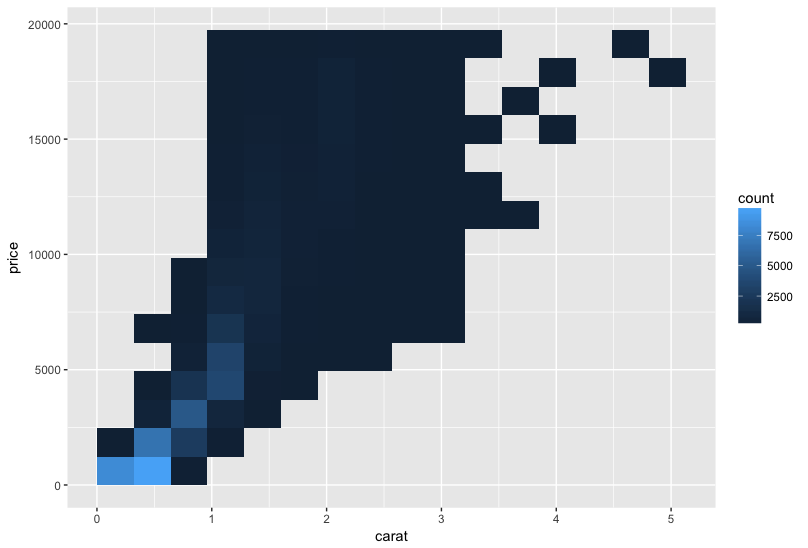
\includegraphics[scale=1 ]{ilu/bg57.png}\end{center}\end{figure}
\begin{lstlisting}[language=html]
# Specify the width of bins
> c + geom_bin2d(binwidth = c(1,1000))
\end{lstlisting}
\begin{figure}[H]\begin{center}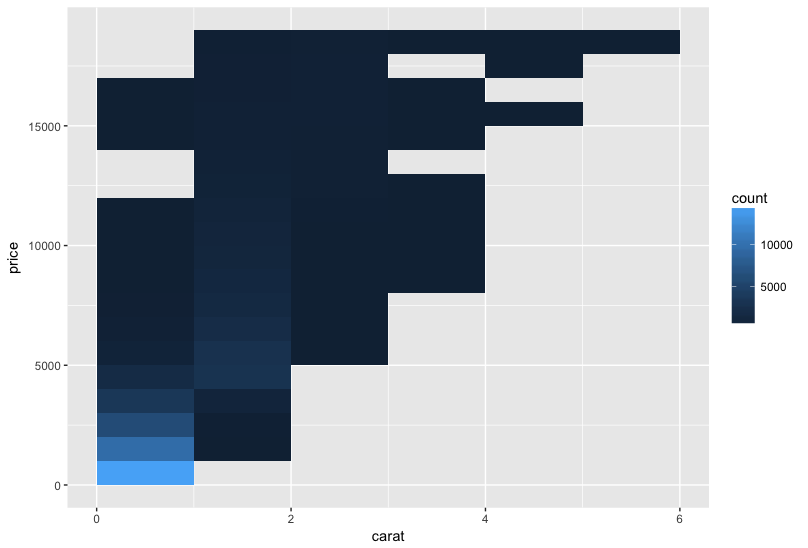
\includegraphics[scale=1 ]{ilu/bg58.png}\end{center}\end{figure}
\begin{lstlisting}[language=html]
> c + stat_bin_2d()
\end{lstlisting}
\begin{figure}[H]\begin{center}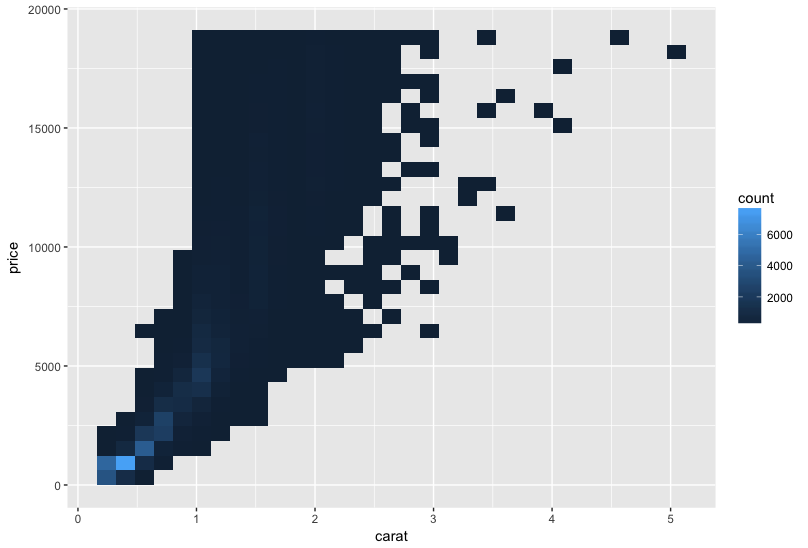
\includegraphics[scale=1 ]{ilu/bg59.png}\end{center}\end{figure}
\begin{lstlisting}[language=html]
> c + stat_summary_2d(aes(z = depth))
\end{lstlisting}
\begin{figure}[H]\begin{center}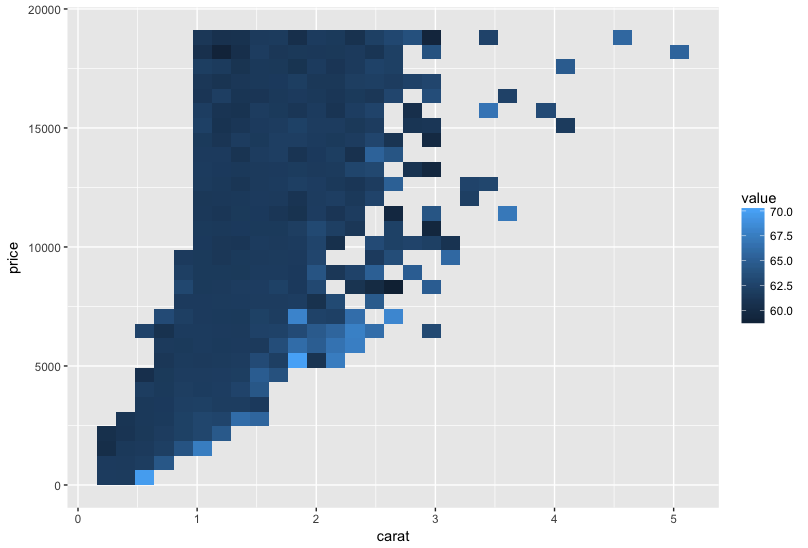
\includegraphics[scale=1 ]{ilu/bg60.png}\end{center}\end{figure}
\begin{lstlisting}[language=html]
# Add hexagon bining
#geom_hex()
# stat_bin_hex(), stat_summary_hex()
# alpha, color, fill, size
> install.packages("hexbin")
> library(hexbin)

> c + geom_hex()
\end{lstlisting}
\begin{figure}[H]\begin{center}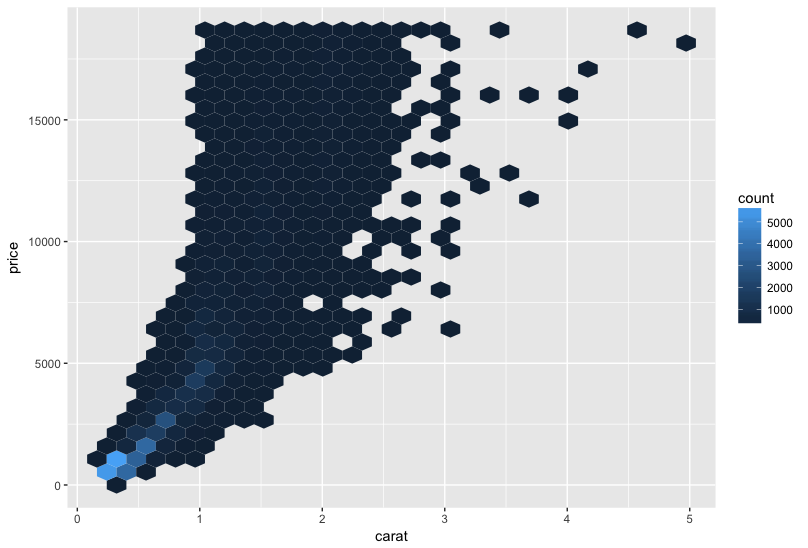
\includegraphics[scale=1 ]{ilu/bg61.png}\end{center}\end{figure}
\begin{lstlisting}[language=html]
# Change the number of bins
> c + geom_hex(bins = 10)
\end{lstlisting}
\begin{figure}[H]\begin{center}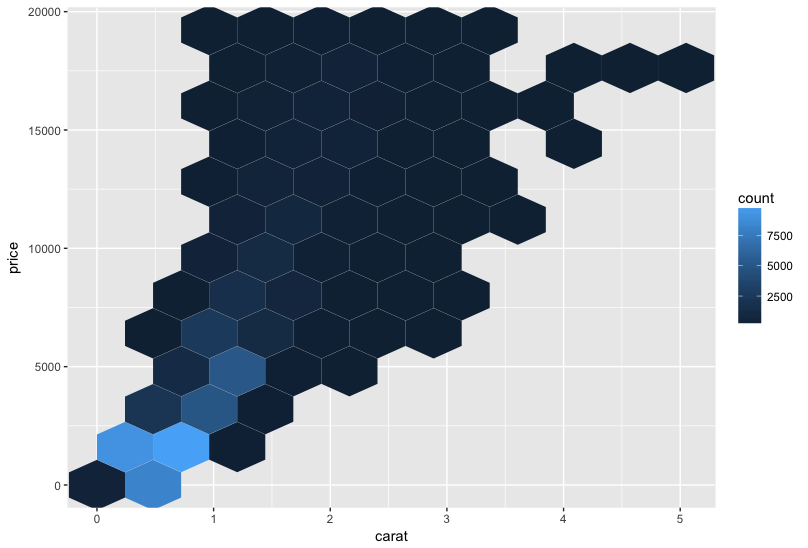
\includegraphics[scale=1 ]{ilu/bg62.png}\end{center}\end{figure}
\begin{lstlisting}[language=html]
> c + stat_bin_hex()
\end{lstlisting}
\begin{figure}[H]\begin{center}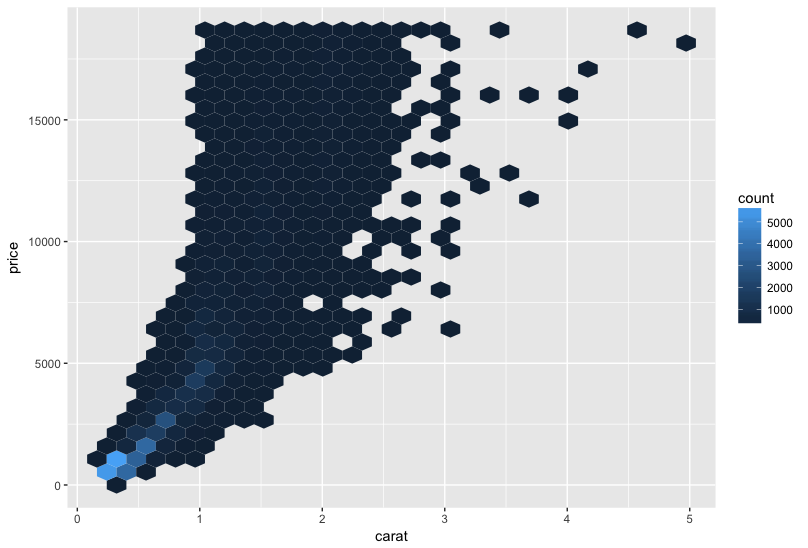
\includegraphics[scale=1 ]{ilu/bg63.png}\end{center}\end{figure}
\begin{lstlisting}[language=html]
> c + stat_summary_hex(aes(z = depth))
\end{lstlisting}
\begin{figure}[H]\begin{center}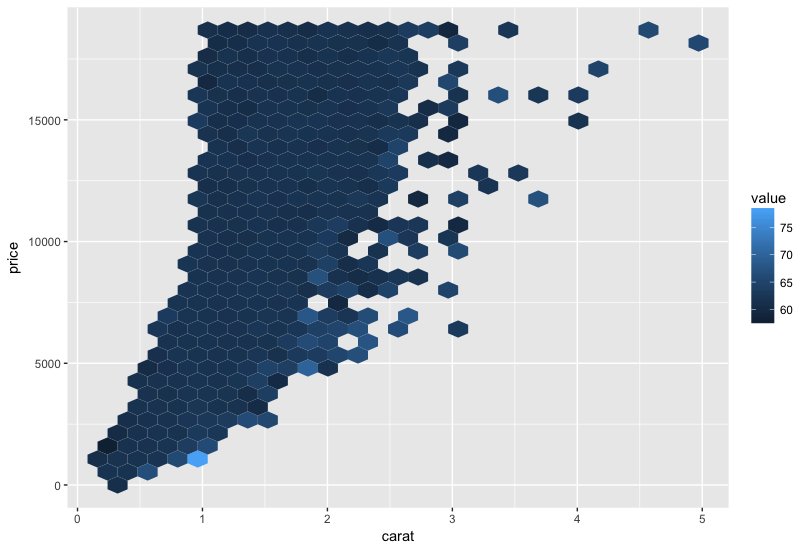
\includegraphics[scale=1 ]{ilu/bg64.png}\end{center}\end{figure}
\begin{lstlisting}[language=html]
# 2D density estimation
# geom_density_2d()
# stat_density_2d()
# alpha, color, linetype, size

# Scatter plot
> sp <- ggplot(faithful, aes(x = eruptions, y = waiting))
> select(faithful, eruptions, waiting)
# A tibble: 272 x 2
   eruptions waiting
 *     <dbl>   <dbl>
 1     3.600      79
 2     1.800      54
 3     3.333      74
 4     2.283      62
 5     4.533      85
 6     2.883      55
 7     4.700      88
 8     3.600      85
 9     1.950      51
10     4.350      85
# ... with 262 more rows
\end{lstlisting}

\begin{lstlisting}[language=html]
# Default plot
> sp + geom_density_2d(color = "#E7B800")
\end{lstlisting}
\begin{figure}[H]\begin{center}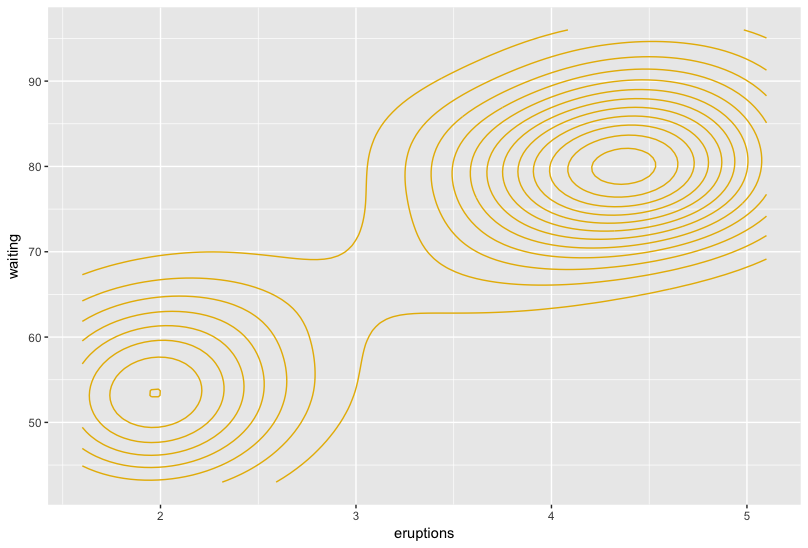
\includegraphics[scale=1 ]{ilu/bg65.png}\end{center}\end{figure}
\begin{lstlisting}[language=html]
# Add points
> sp + geom_point(color = "#00AFBB") + geom_density_2d(color = "#E7B800")
\end{lstlisting}
\begin{figure}[H]\begin{center}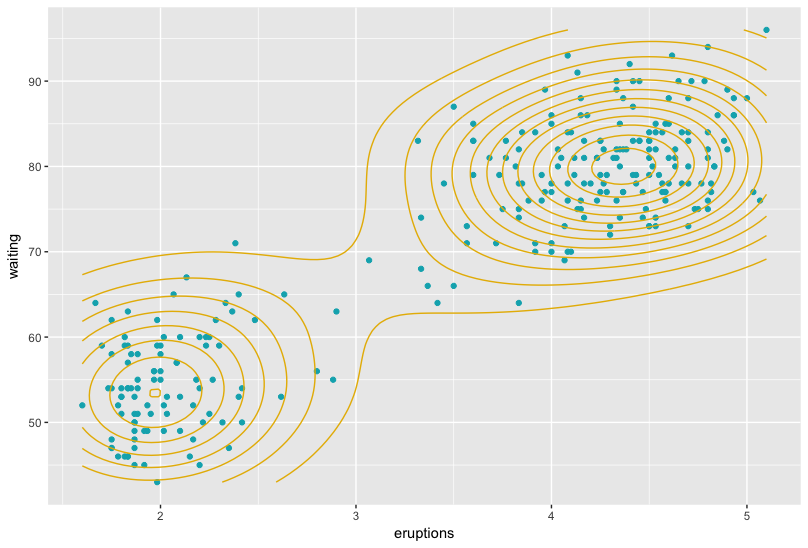
\includegraphics[scale=1 ]{ilu/bg66.png}\end{center}\end{figure}
\begin{lstlisting}[language=html]
# Use stat_density_2d with geom = "polygon"
sp + geom_point() + stat_density_2d(aes(fill = ..level..), geom = "polygon")
\end{lstlisting}
\begin{figure}[H]\begin{center}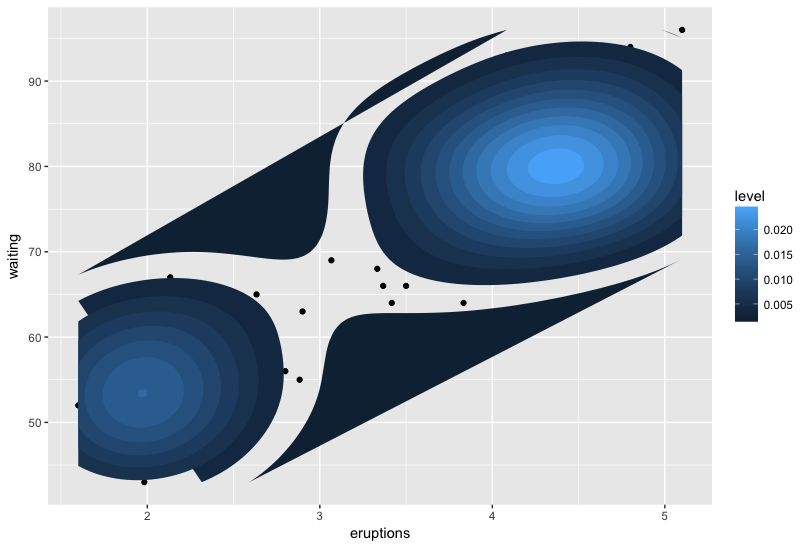
\includegraphics[scale=1 ]{ilu/bg67.png}\end{center}\end{figure}
\begin{lstlisting}[language=html]
# Change the gradient color
> sp + geom_point() + stat_density_2d(aes(fill = ..level..), geom = "polygon") + scale_fill_gradient(low = "#00AFBB", high = "#FC3E07")
\end{lstlisting}
\begin{figure}[H]\begin{center}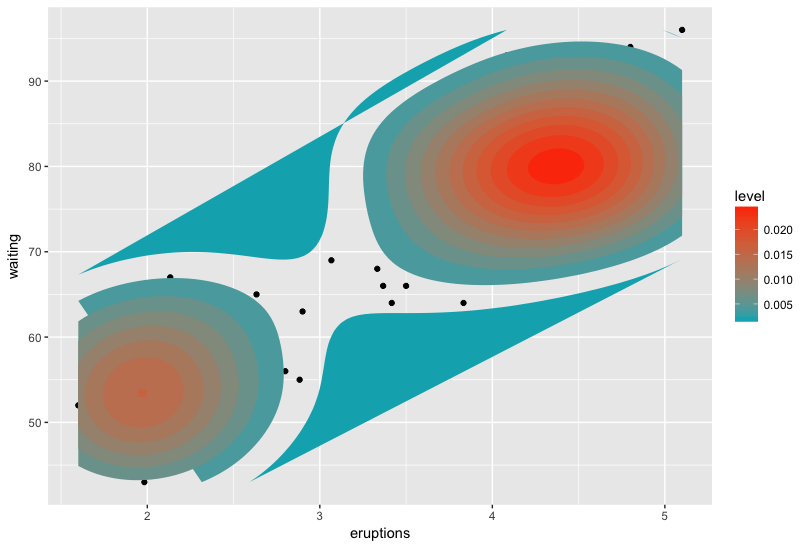
\includegraphics[scale=1 ]{ilu/bg68.png}\end{center}\end{figure}
\begin{lstlisting}[language=html]
# Gradient
\end{lstlisting}
\subsection{Two variables: Discrete X, Discrete Y}

\textbf{geom_jitter\newline
alpha, color, fill, shape, size}
\begin{lstlisting}[language=html]
> ggplot(diamonds, aes(cut, color)) + geom_jitter(aes(color = cut), size = 0.5)
\end{lstlisting}
\begin{figure}[H]\begin{center}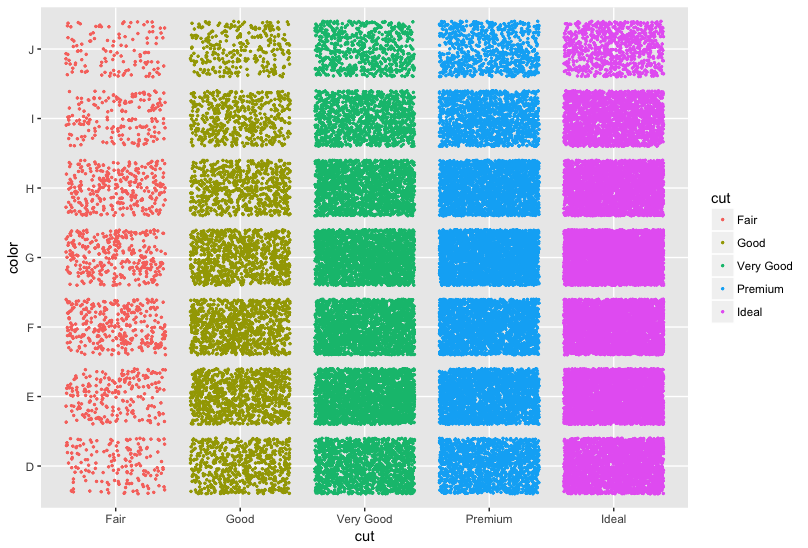
\includegraphics[scale=1 ]{ilu/bg69.png}\end{center}\end{figure}
\begin{lstlisting}[language=html]
> select(diamonds, cut, color)
# A tibble: 53,940 x 2
         cut color
       <ord> <ord>
 1     Ideal     E
 2   Premium     E
 3      Good     E
 4   Premium     I
 5      Good     J
 6 Very Good     J
 7 Very Good     I
 8 Very Good     H
 9      Fair     E
10 Very Good     H
# ... with 53,930 more rows
\end{lstlisting}

\section{Plot Two Variables - X & Y: Discrete X and Continuous Y}
\begin{itemize}
  \item geom\_boxplot()
  \item geom\_violin()
  \item geom\_dotplot()
  \item geom\_jitter()
  \item geom\_line()
  \item geom\_bar()

\end{itemize}

\begin{lstlisting}[language=html]
> data("ToothGrowth")
> ToothGrowth$dose <- as.factor(ToothGrowth$dose)
> ToothGrowth <- as_data_frame(ToothGrowth)
> ToothGrowth
# A tibble: 60 x 3
     len   supp   dose
   <dbl> <fctr> <fctr>
 1   4.2     VC    0.5
 2  11.5     VC    0.5
 3   7.3     VC    0.5
 4   5.8     VC    0.5
 5   6.4     VC    0.5
 6  10.0     VC    0.5
 7  11.2     VC    0.5
 8  11.2     VC    0.5
 9   5.2     VC    0.5
10   7.0     VC    0.5
# ... with 50 more rows
\end{lstlisting}
\textcolor{white}{.}\newline
\begin{lstlisting}[language=html]
## Chargement de e
e <- ggplot(ToothGrowth, aes(x = dose, y = len))
\end{lstlisting}
\subsection{Box Plots}

\textbf{alpha, color, linetype, shape, size, fill}\newline
\begin{lstlisting}[language=html]
> geom_boxplot(outlier.colour = "black", outlier.shape = 16, outlier.size = 2, notch = FALSE)
\end{lstlisting}
\textcolor{white}{.}\newline
\begin{lstlisting}[language=html]
# Basic box plot
> e + geom_boxplot()
\end{lstlisting}
\begin{figure}[H]\begin{center}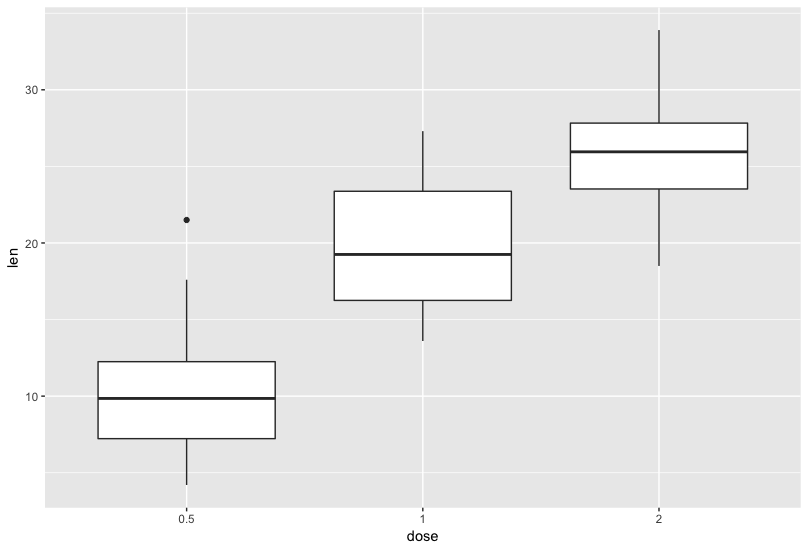
\includegraphics[scale=1 ]{ilu/bg70.png}\end{center}\end{figure}
\begin{lstlisting}[language=html]
# Rotate the box plot
> e + geom_boxplot() + coord_flip()
\end{lstlisting}
\begin{figure}[H]\begin{center}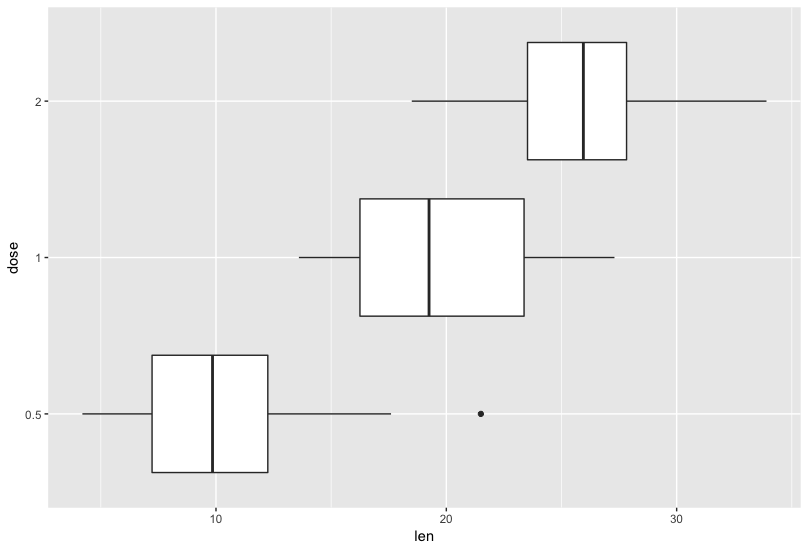
\includegraphics[scale=1 ]{ilu/bg71.png}\end{center}\end{figure}
\begin{lstlisting}[language=html]
# Notched box plot
> e + geom_boxplot(notch = TRUE)
\end{lstlisting}
\begin{figure}[H]\begin{center}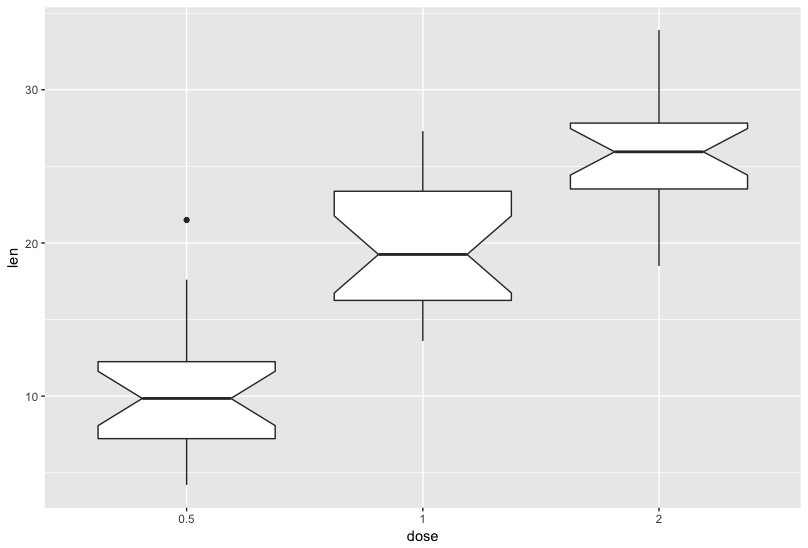
\includegraphics[scale=1 ]{ilu/bg72.png}\end{center}\end{figure}
\begin{lstlisting}[language=html]
# Box plot with mean points
> e + geom_boxplot() + stat_summary(fun.y = mean, geom = "point", shape = 18, size = 4, color = "blue")
\end{lstlisting}
\begin{figure}[H]\begin{center}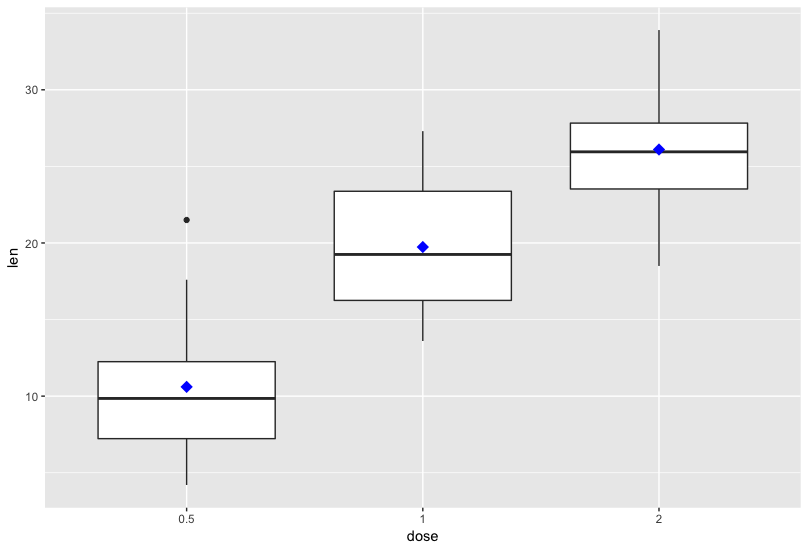
\includegraphics[scale=1 ]{ilu/bg73.png}\end{center}\end{figure}
\begin{lstlisting}[language=html]
# chose which item to display
> e + geom_boxplot() + scale_x_discrete(limits = c("0.5", "2"))
\end{lstlisting}
\begin{figure}[H]\begin{center}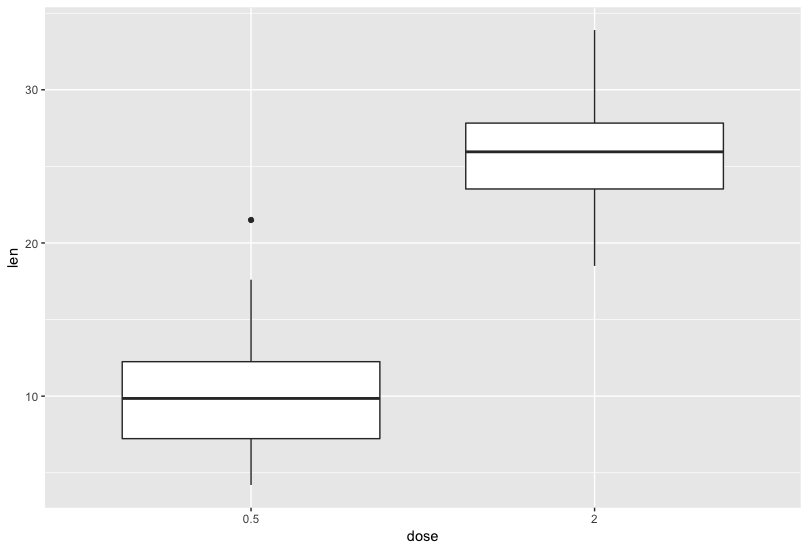
\includegraphics[scale=1 ]{ilu/bg74.png}\end{center}\end{figure}
\begin{lstlisting}[language=html]
# change default order of items
> e + geom_boxplot() + scale_x_discrete(limits = c("2", "0.5", "1"))
\end{lstlisting}
\begin{figure}[H]\begin{center}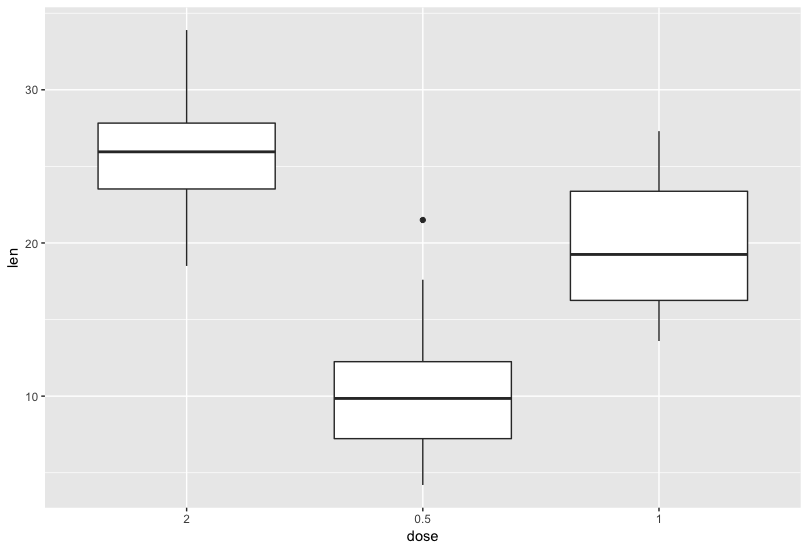
\includegraphics[scale=1 ]{ilu/bg75.png}\end{center}\end{figure}
\begin{lstlisting}[language=html]
> e + stat_boxplot(coeff = 1.5)
## Warning: Ignoring unknown parameters: coeff
\end{lstlisting}
\begin{figure}[H]\begin{center}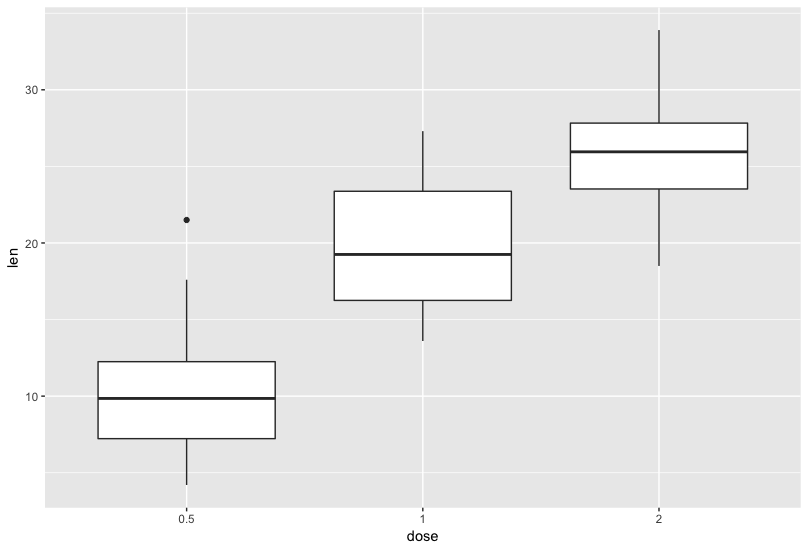
\includegraphics[scale=1 ]{ilu/bg76.png}\end{center}\end{figure}

\textbf{Change the color by group :} box plot outline and fill colors can be automatically controlled by the levels of the grouping variable \textit{dose}
\begin{lstlisting}[language=html]
# Use single color
> e + geom_boxplot(color = "black", fill = "steelblue")
\end{lstlisting}
\begin{figure}[H]\begin{center}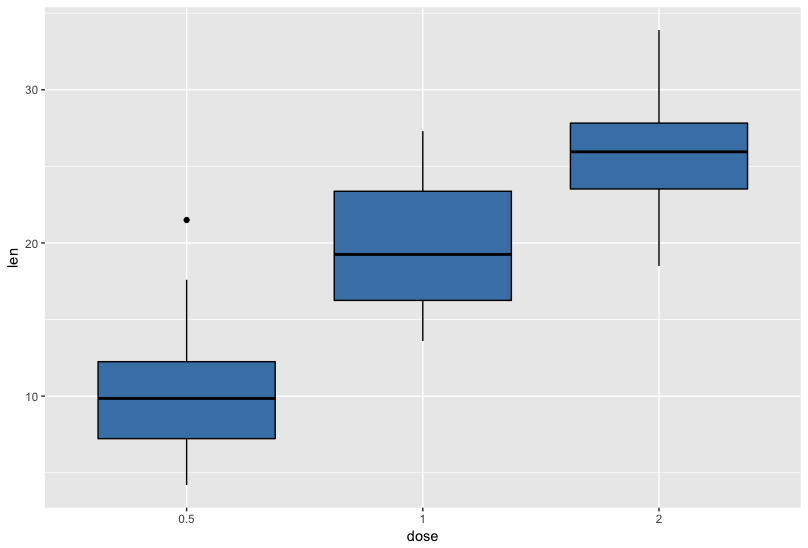
\includegraphics[scale=1 ]{ilu/bg77.png}\end{center}\end{figure}
\begin{lstlisting}[language=html]
# Change outline colors by dose (groups)
> e + geom_boxplot(aes(color = dose))
\end{lstlisting}
\begin{figure}[H]\begin{center}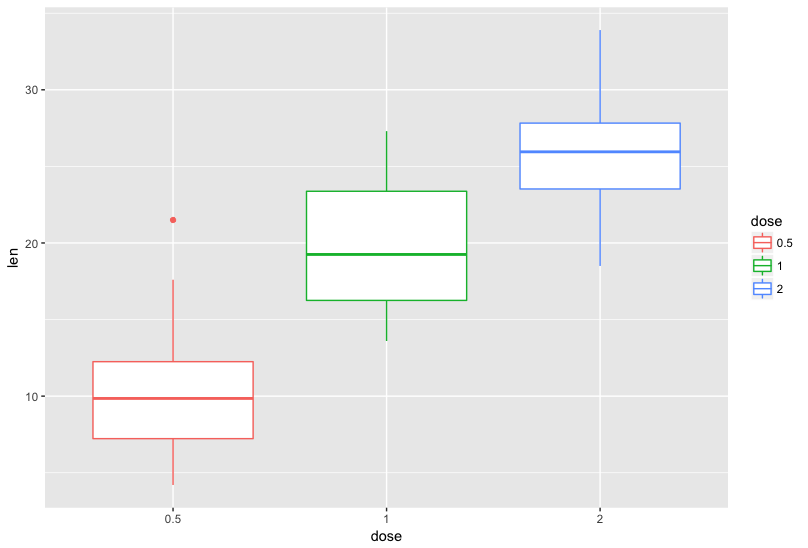
\includegraphics[scale=1 ]{ilu/bg78.png}\end{center}\end{figure}
\begin{lstlisting}[language=html]
# Change the fill color by dose (groups)
> e + geom_boxplot(aes(fill = dose))
\end{lstlisting}
\begin{figure}[H]\begin{center}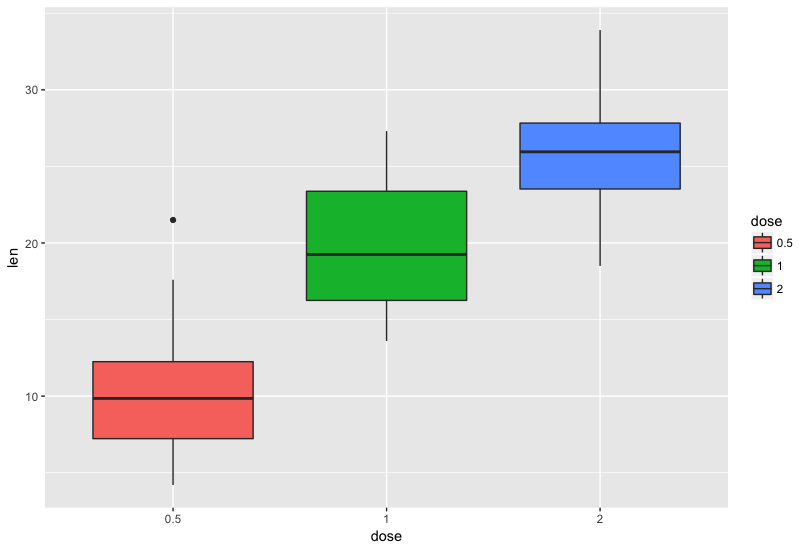
\includegraphics[scale=1 ]{ilu/bg79.png}\end{center}\end{figure}
\begin{lstlisting}[language=html]
# Change munually outline colors:
# Use custom color palettes
> e2 <- e + geom_boxplot(aes(color = dose)) + theme_minimal()
> e2 + scale_color_manual(values = c("#999999", "#E69F00", "#56B4E9"))
\end{lstlisting}
\begin{figure}[H]\begin{center}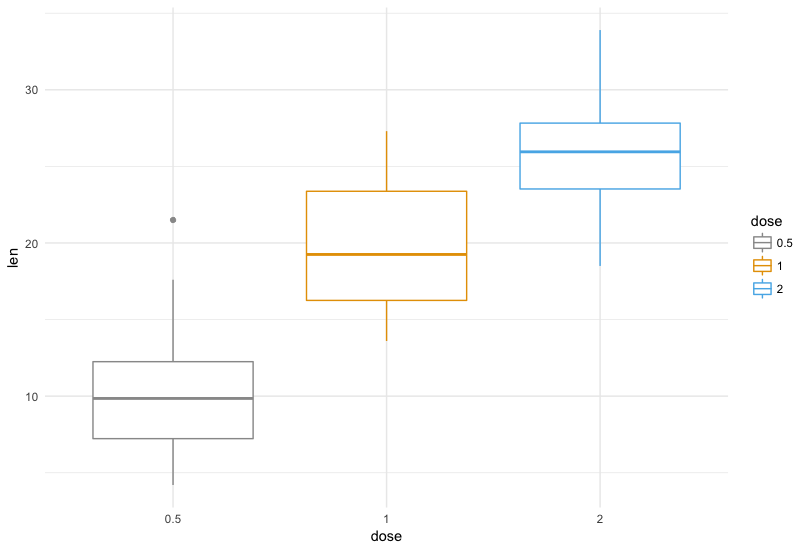
\includegraphics[scale=1 ]{ilu/bg80.png}\end{center}\end{figure}
\begin{lstlisting}[language=html]
# Use brewer color palettes
> e2 + scale_color_brewer(palette  = "Dark2")
\end{lstlisting}
\begin{figure}[H]\begin{center}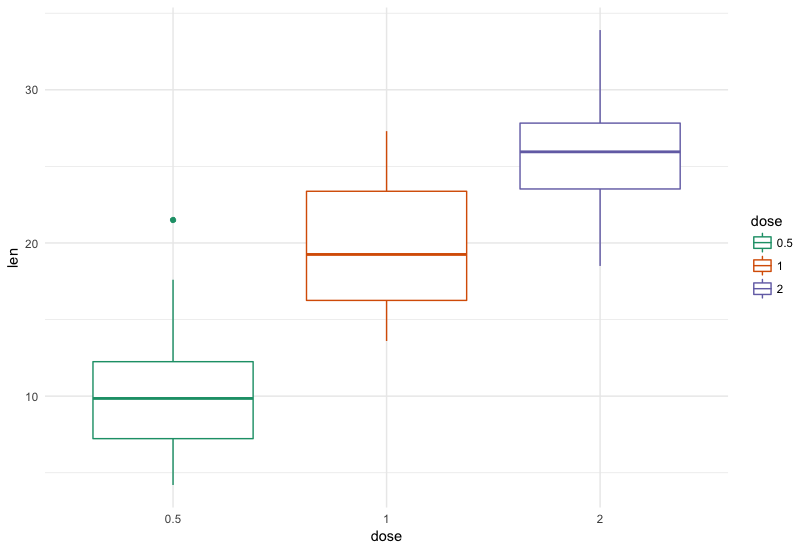
\includegraphics[scale=1 ]{ilu/bg81.png}\end{center}\end{figure}
\begin{lstlisting}[language=html]
# Use grey scale
> e2 + scale_color_grey()
\end{lstlisting}
\begin{figure}[H]\begin{center}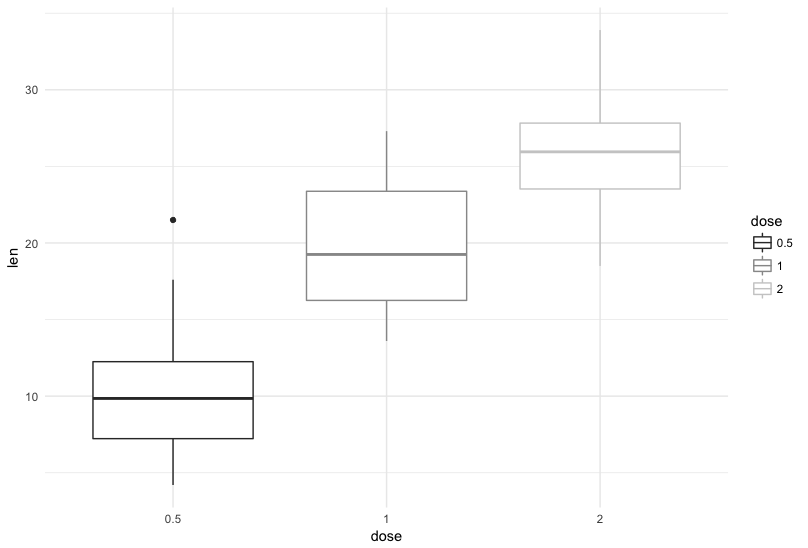
\includegraphics[scale=1 ]{ilu/bg82.png}\end{center}\end{figure}
\begin{lstlisting}[language=html]
## Change manually by fill color
# Use the custom color palettes
> e3 <- e + geom_boxplot(aes(fill = dose)) + theme_minimal()
> e3 + scale_fill_manual(values = c("#999999", "#E69F00", "#56B4E9"))
\end{lstlisting}
\begin{figure}[H]\begin{center}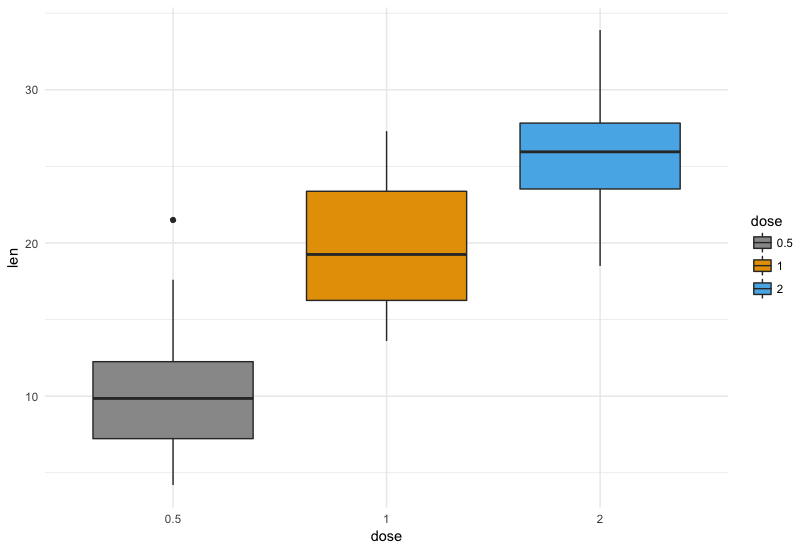
\includegraphics[scale=1 ]{ilu/bg83.png}\end{center}\end{figure}
\begin{lstlisting}[language=html]
# Use brewer color palettes
> e3 + scale_fill_brewer(palette = "Dark2")
\end{lstlisting}
\begin{figure}[H]\begin{center}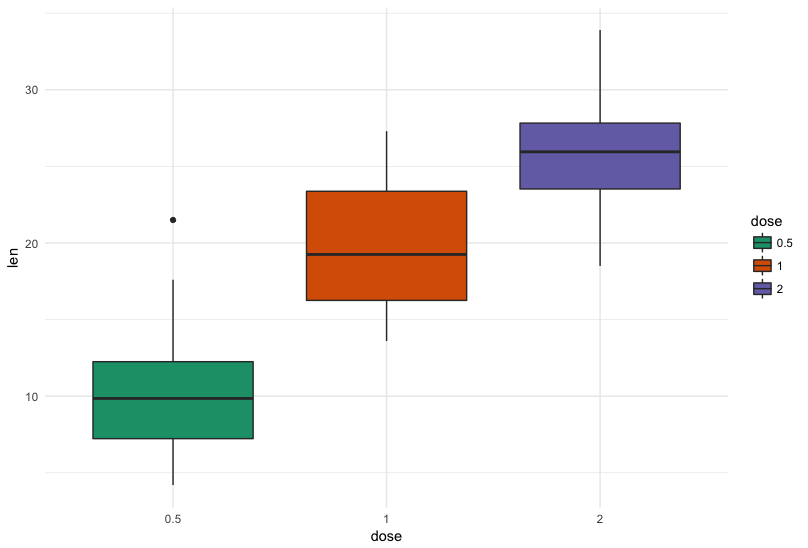
\includegraphics[scale=1 ]{ilu/bg84.png}\end{center}\end{figure}
\begin{lstlisting}[language=html]
# Use grey color
> e3 + scale_fill_grey()
\end{lstlisting}
\begin{figure}[H]\begin{center}\includegraphics[scale=1 ]{ilu/bg85.png}\end{center}\end{figure}

\textbf{Boxplot with multiple groups : } The grouping variable \textit{dose} and \textit{supp} are used :
\begin{lstlisting}[language=html]
# Change box plot colors by groups
e + geom_boxplot(aes(fill = supp))
\end{lstlisting}
\begin{figure}[H]\begin{center}\includegraphics[scale=1 ]{ilu/bg86.png}\end{center}\end{figure}
\begin{lstlisting}[language=html]
# Change the position
e + geom_boxplot(aes(fill = supp), position = position_dodge(1.1))
\end{lstlisting}
\begin{figure}[H]\begin{center}\includegraphics[scale=1 ]{ilu/bg87.png}\end{center}\end{figure}
\begin{lstlisting}[language=html]
# Change the fill color
e + geom_boxplot(aes(fill = supp), position = position_dodge(1.1)) + scale_fill_brewer("BrBG")
\end{lstlisting}
\begin{figure}[H]\begin{center}\includegraphics[scale=1 ]{ilu/bg88.png}\end{center}\end{figure}

\subsection{Violin Plots}
Violin plots is similar to boxplot, except that they also show the kernel probability density of the data at different values. Tipically, violin plots will include a marker for the median of the data and a box indicating the interquartile range, as in standard boxplots.\newline
\\
\textbf{alpha, color, fill, linetype, size, and fill}
\begin{lstlisting}[language=html]
# Basic plot
> e + geom_violin()
\end{lstlisting}
\begin{figure}[H]\begin{center}\includegraphics[scale=1 ]{ilu/bg89.png}\end{center}\end{figure}
\begin{lstlisting}[language=html]
# Rotate the violin plot
> e + geom_violin() + coord_flip()
\end{lstlisting}
\begin{figure}[H]\begin{center}\includegraphics[scale=1 ]{ilu/bg90.png}\end{center}\end{figure}
\begin{lstlisting}[language=html]
# Set trim argument to FALSE
> e + geom_violin(trim = FALSE, fill = "steelblue")
\end{lstlisting}
\begin{figure}[H]\begin{center}\includegraphics[scale=1 ]{ilu/bg91.png}\end{center}\end{figure}

\textbf{Add summary statistics : } Funtion stat\_summary() can be used to add mean/median points and more on a violin plot
\begin{lstlisting}[language=html]
# Add mean and median points: use fun.y = mean or fun.y = median
e + geom_violin(trim = FALSE) + stat_summary(fun.y = mean, geom = "point", shape = 23, size = 2, color = "blue")
\end{lstlisting}

\begin{figure}[H]\begin{center}\includegraphics[scale=1 ]{ilu/bg92.png}\end{center}\end{figure}
\begin{lstlisting}[language=html]
# Add mean points +/- SD
# Use geom = "pointrange" or geom = "crossbar"
> library("Hmisc") ## stat_summary
> e + geom_violin(trim = FALSE) + stat_summary(fun.data = "mean_sdl", fun.args = list(mult = 1), geom = "pointrange", color = "red")
\end{lstlisting}
\begin{figure}[H]\begin{center}\includegraphics[scale=1 ]{ilu/bg93.png}\end{center}\end{figure}


The function \textit{mean\_sdl} is used for adding mean and standard deviation. It computes the mean plus or minus a constant times the standard deviation. The constant is specified using the argument\textit{mult} (\textit{mult} = 1). Default \textit{mult = 2}.\newline
The mean $\pm$ SD can be added as crossbar or a pointrange. 
\begin{lstlisting}[language=html]
# Combine with box plot to add median and quartiles
> e + geom_violin(trim = FALSE) + geom_boxplot(width = 0.2)
\end{lstlisting}
\begin{figure}[H]\begin{center}\includegraphics[scale=1 ]{ilu/bg94.png}\end{center}\end{figure}

\textbf{Change colors by groups : } The color and fill can be automatically controlled by the levels  of the grouping variable dose. 
\begin{lstlisting}[language=html]
# Change the outline colors by dose (groups)
> e + geom_violin(aes(color = dose), trim = FALSE)
\end{lstlisting}
\begin{figure}[H]\begin{center}\includegraphics[scale=1 ]{ilu/bg95.png}\end{center}\end{figure}
\begin{lstlisting}[language=html]
# Change the fill color by dose
> e  + geom_violin(aes(fill = dose), trim = FALSE)
\end{lstlisting}
\begin{figure}[H]\begin{center}\includegraphics[scale=1 ]{ilu/bg96.png}\end{center}\end{figure}
\begin{lstlisting}[language=html]
# Change outline and fill color manually.
> e2 <- e + geom_violin(aes(color = dose), trim = FALSE) + theme_minimal()
> e2 + scale_color_brewer(palette = "Dark2")
\end{lstlisting}
\begin{figure}[H]\begin{center}\includegraphics[scale=1 ]{ilu/bg97.png}\end{center}\end{figure}
\begin{lstlisting}[language=html]
# Change manually fill colors
> e3 <- e + geom_violin(aes(fill = dose), trim = FALSE) + theme_minimal()
> e3 + scale_fill_brewer(palette = "Dark2")
\end{lstlisting}
\begin{figure}[H]\begin{center}\includegraphics[scale=1 ]{ilu/bg98.png}\end{center}\end{figure}

\begin{lstlisting}[language=html]
## Violin plot with multiple groups
# Change the color by groups
> e + geom_violin(aes(fill = supp), trim = FALSE)
\end{lstlisting}
\begin{figure}[H]\begin{center}\includegraphics[scale=1 ]{ilu/bg99.png}\end{center}\end{figure}
\begin{lstlisting}[language=html]
# Change fill colors
> e + geom_violin(aes(fill = supp), trim = FALSE) + scale_fill_brewer(palette = "Dark2")
\end{lstlisting}
\begin{figure}[H]\begin{center}\includegraphics[scale=1 ]{ilu/bg100.png}\end{center}\end{figure}

\subsection{Dot plots}
geom_dotplot(), stat_summary() (package : "Hmisc")\newline
\\
\textbf{alpha, color, dotsize and fill}
\begin{lstlisting}[language=html]
#Basic dot plot
> e + geom_dotplot(binaxis ="y", stackdir = "center")
\end{lstlisting}
\begin{figure}[H]\begin{center}\includegraphics[scale=1 ]{ilu/bg101.png}\end{center}\end{figure}
\begin{lstlisting}[language=html]
# Change dotsize and stack ratio
> e + geom_dotplot(binaxis = "y", stackdir = "center", stackratio = 1.5, dotsize = 1.1)
\end{lstlisting}
\begin{figure}[H]\begin{center}\includegraphics[scale=1 ]{ilu/bg102.png}\end{center}\end{figure}

\textit{stat\_summary()} can be used to add mean/median points and more on a violin plot.
\begin{lstlisting}[language=html]
# Add mean and median points: use fun.y = mean or fun.y = median
> e + geom_dotplot(binaxis = "y", stackdir = "center") + stat_summary(fun.y = mean, geom = "point", shape = 18, size = 3, color = "red")
\end{lstlisting}
\begin{figure}[H]\begin{center}\includegraphics[scale=1 ]{ilu/bg103.png}\end{center}\end{figure}
\begin{lstlisting}[language=html]
# Add mean points with +/- SD
# Use geom = "pointrange" or geom = "crossbar"
> e + geom_dotplot(binaxis = "y", stackdir = "center") + stat_summary(fun.data = "mean_sdl", fun.args = list(mult = 1), geom = "pointrange", color = "red")
\end{lstlisting}
\begin{figure}[H]\begin{center}\includegraphics[scale=1 ]{ilu/bg104.png}\end{center}\end{figure}

Combine with box plot and dot plot:
\begin{lstlisting}[language=html]
# Combine with boxplot
> e + geom_boxplot() + geom_dotplot(binaxis = "y", stackdir ="center")
\end{lstlisting}
\begin{figure}[H]\begin{center}\includegraphics[scale=1 ]{ilu/bg105.png}\end{center}\end{figure}
%%%%%%%%%%%%%%%%%%%%%%%%%%%%%%%%%%%%%%%%%%%%%%%%%%%%%%%%%%%%%%%%%%%%%%%%%%%%%%
\begin{lstlisting}[language=html]
# Combine with violin plot
> e + geom_violin(trim = FALSE) + geom_dotplot(binaxis = "y", stackdir ="center")
\end{lstlisting}
\begin{figure}[H]\begin{center}\includegraphics[scale=1 ]{ilu/bg106.png}\end{center}\end{figure}
\begin{lstlisting}[language=html]
# Dotplot + violin plot + stat summary
> e + geom_violin(trim = FALSE) + geom_dotplot(binaxis = "y", stackdir ="center") + stat_summary(fun.data = "mean_sdl", fun.args = list(mult = 1), geom = "pointrange", color = "red", shape = 11)
\end{lstlisting}
\begin{figure}[H]\begin{center}\includegraphics[scale=1 ]{ilu/bg107.png}\end{center}\end{figure}

Use scale to change the outlien and fill color automatically controlled byt the levels of the grouping variable dose : 
\begin{itemize}
  \item scale\_color\_munual(), scale\_color\_brewer(), scale\_color\_grey()
  \item scale\_fill\_munual(), sclae\_fill\_brewer(), scale\_fill\_grey()
\end{itemize}
 
\begin{figure}[H]\begin{center}\includegraphics[scale=1 ]{ilu/bg108.png}\end{center}\end{figure} 

Dotplot with multiple groups, just like boxplot and violin plot

\subsection{Stripcharts}
Stripecharts are also known as one dimensional scatter plots. These plots are suitable compared to box plot when sample sizes are small.\newline
\textit{geom\_jitter(), stat\_summary()}.\newline
\\
\textbf{alpha, color, size and fill}
\begin{lstlisting}[language=html]
> e <- ggplot(ToothGrowth, aes(x = dose, y = len))
> e + geom_jitter()
\end{lstlisting}
\begin{figure}[H]\begin{center}\includegraphics[scale=1 ]{ilu/bg109.png}\end{center}\end{figure} 
\begin{lstlisting}[language=html]
# Change the position
# 0.2 is the degree of jitter in x direction
> e + geom_jitter(position = position_jitter(0.2))
\end{lstlisting}
\begin{figure}[H]\begin{center}\includegraphics[scale=1 ]{ilu/bg110.png}\end{center}\end{figure} 
\begin{lstlisting}[language=html]
# Change point shapes and size
> e  + geom_boxplot()+ geom_jitter(position = position_jitter(0.2), shape = 11, size = 1.2)
\end{lstlisting}
\begin{figure}[H]\begin{center}\includegraphics[scale=1 ]{ilu/bg111.png}\end{center}\end{figure} 
\begin{lstlisting}[language=html]
# Add summary statistics
# Add mean or median point
> e + geom_jitter(position = position_jitter(0.2)) + stat_summary(fun.y = mean, geom = "point", shape = 18, size = 3, color = "red")
\end{lstlisting}
\begin{figure}[H]\begin{center}\includegraphics[scale=1 ]{ilu/bg112.png}\end{center}\end{figure} 
\begin{lstlisting}[language=html]
# use geom = "pointrange"
> e + geom_jitter(position = position_jitter(0.2)) + stat_summary(fun.data = "mean_sdl", fun.args = list(mult = 1), shape = 18, color = "red")
\end{lstlisting}
\begin{figure}[H]\begin{center}\includegraphics[scale=1 ]{ilu/bg113.png}\end{center}\end{figure}
\begin{lstlisting}[language=html]
# Combine with boxplot and violin plot
> e + geom_violin(trim = FALSE) + geom_jitter(position = position_jitter(0.1)) + stat_summary(fun.data = "mean_sdl", fun.args = list(mult = 1), shape = 18, color = "red")
\end{lstlisting}
\begin{figure}[H]\begin{center}\includegraphics[scale=1 ]{ilu/bg114.png}\end{center}\end{figure}
\begin{lstlisting}[language=html]
# Change point shape by group
> e + geom_jitter(aes(shape = dose), position = position_jitter(0.2)) + scale_shape_manual(values = c(1,17,19))
\end{lstlisting}
\begin{figure}[H]\begin{center}\includegraphics[scale=1 ]{ilu/bg115.png}\end{center}\end{figure}
\begin{lstlisting}[language=html]
# Change color by groups
> e + geom_jitter(aes(color = dose, shape = dose), position = position_jitter(0.2)) + theme_minimal()
\end{lstlisting}
\begin{figure}[H]\begin{center}\includegraphics[scale=1 ]{ilu/bg116.png}\end{center}\end{figure}

\textbf{Change the outlien and fill color by scale : } Stripchar with multiple groups.
\begin{lstlisting}[language=html]
#Change colors and shapes by groups
> e + geom_jitter(aes(color = supp, shape = supp), position = position_jitter(0.2))
\end{lstlisting}
\begin{figure}[H]\begin{center}\includegraphics[scale=1 ]{ilu/bg117.png}\end{center}\end{figure}
\begin{lstlisting}[language=html]
# Add boxplot
> e + geom_boxplot(aes(color = supp), position = position_dodge()) + geom_jitter(aes(color = supp, shape = supp), position = position_jitter(0.2)) + theme_minimal()
\end{lstlisting}
\begin{figure}[H]\begin{center}\includegraphics[scale=1 ]{ilu/bg118.png}\end{center}\end{figure}


\subsection{Line plots}
In a line graph, observations are ordered by x value and connected.\newline
x value can be :
\begin{itemize}
  \item date: for a time series data
  \item texts
  \item discrete numeric values
  \item continuous numeric values
\end{itemize}
\textit{geom\_line(), geom\_path(), geom\_step()}.\newline
\\
\textbf{alpha, color, linetype and size}
\begin{lstlisting}[language=html]
> df <- data.frame(dose = c("D0.5", "D1", "D2"), len = c(4.2,10, 29.5))
> df2 <- data.frame(supp = rep(c("VC", "OJ"), each = 3), dose = rep(c("D0.5", "D1", "D2"),2 ), len = c(6.8, 15, 33, 4.2, 10, 29.5))
> p<- ggplot(data = df, aes(x = dose, y = len, group = 1))
> p + geom_line() + geom_point()
\end{lstlisting}
\begin{figure}[H]\begin{center}\includegraphics[scale=1 ]{ilu/bg119.png}\end{center}\end{figure}
\begin{lstlisting}[language=html]
# Change the line color and line type
> p + geom_line(linetype = "dashed", color = "steelblue") + geom_point(color = "steelblue")
\end{lstlisting}
\begin{figure}[H]\begin{center}\includegraphics[scale=1 ]{ilu/bg120.png}\end{center}\end{figure}
\begin{lstlisting}[language=html]
# use geom_step()
> p + geom_step() + geom_point()
\end{lstlisting}
\begin{figure}[H]\begin{center}\includegraphics[scale=1 ]{ilu/bg121.png}\end{center}\end{figure}
\begin{lstlisting}[language=html]
# use paht
> p + geom_path() 
\end{lstlisting}
\begin{figure}[H]\begin{center}\includegraphics[scale=1 ]{ilu/bg122.png}\end{center}\end{figure}
\begin{lstlisting}[language=html]
# Line plot with multiple groups
# line tpye and point shape automatically controlled by groups.
> p <- ggplot(df2, aes(x = dose, y= len, group = supp))
> p + geom_line(aes(linetype = supp)) + geom_point(aes(shape = supp))
\end{lstlisting}
\begin{figure}[H]\begin{center}\includegraphics[scale=1 ]{ilu/bg123.png}\end{center}\end{figure}
\begin{lstlisting}[language=html]
# Change the line type, point shapes and colors
> p + geom_line(aes(linetype = supp, color = supp)) + geom_point(aes(shape = supp, color = supp)) + scale_color_brewer(palette = "Dark2")
\end{lstlisting}
\begin{figure}[H]\begin{center}\includegraphics[scale=1 ]{ilu/bg124.png}\end{center}\end{figure}
\begin{lstlisting}[language=html]
# X-axis is date; use economics
> head(economics)
# A tibble: 6 x 6
        date   pce    pop psavert uempmed unemploy
      <date> <dbl>  <int>   <dbl>   <dbl>    <int>
1 1967-07-01 507.4 198712    12.5     4.5     2944
2 1967-08-01 510.5 198911    12.5     4.7     2945
3 1967-09-01 516.3 199113    11.7     4.6     2958
4 1967-10-01 512.9 199311    12.5     4.9     3143
5 1967-11-01 518.1 199498    12.5     4.7     3066
6 1967-12-01 525.8 199657    12.1     4.8     3018
\end{lstlisting}
\textcolor{white}{.}\newline
\begin{lstlisting}[language=html]
> ggplot(data = economics, aes(x = date, y = pop)) + geom_line()
\end{lstlisting}
\begin{figure}[H]\begin{center}\includegraphics[scale=1 ]{ilu/bg125.png}\end{center}\end{figure}
\begin{lstlisting}[language=html]
# subset data
> ss <- subset(economics, date > as.Date("2006-1-1"))
> ggplot(data = ss, aes(x = date, y = pop)) + geom_line()
\end{lstlisting}
\begin{figure}[H]\begin{center}\includegraphics[scale=1 ]{ilu/bg126.png}\end{center}\end{figure}
\begin{lstlisting}[language=html]
# line size
> ggplot(data = economics, aes(x = date, y = pop, size = unemploy/ pop)) + geom_line()
\end{lstlisting}
\begin{figure}[H]\begin{center}\includegraphics[scale=1 ]{ilu/bg127.png}\end{center}\end{figure}
\begin{lstlisting}[language=html]
# multiple time series data:
# Solution 1
ggplot(economics, aes(x = date)) + geom_line(aes(y = psavert, color = "darkred")) + geom_line(aes(y = uempmed), color = "steelblue", linetype = "twodash") + theme_minimal()
\end{lstlisting}
\begin{figure}[H]\begin{center}\includegraphics[scale=1 ]{ilu/bg128.png}\end{center}\end{figure}
\begin{lstlisting}[language=html]
# Solution 2: melt by date
# Area plot
ggplot(economics, aes(x = date)) + geom_area(aes(y = psavert), fill = "#999999", color = "#999999", alpha = 0.5) + geom_area(aes(y = uempmed), fill = "#E69F00", color = "#E69F00", alpha = 0.5) + theme_minimal()
\end{lstlisting}
\begin{figure}[H]\begin{center}\includegraphics[scale=1 ]{ilu/bg129.png}\end{center}\end{figure}

\subsection{Bar plots}
\textit{geom\_bar()}.\newline
\\
\textbf{alpha, color, fill, linetype and size}
\begin{lstlisting}[language=html]
> df <- data.frame(dose = c("D0.5", "D1", "D2"), len = c(4.2,10, 29.5))
> df2 <- data.frame(supp = rep(c("VC", "OJ"), each = 3), dose = rep(c("D0.5", "D1", "D2"),2 ), len = c(6.8, 15, 33, 4.2, 10, 29.5))
> f <- ggplot(df, aes(x = dose, y = len))
> f + geom_bar(stat = "identity")
\end{lstlisting}
\begin{figure}[H]\begin{center}\includegraphics[scale=1 ]{ilu/bg130.png}\end{center}\end{figure}
\begin{lstlisting}[language=html]
#Change fill color and add labels at the top
> f + geom_bar(stat= "identity", fill = "steelblue") + geom_text(aes(label = len), vjust = -0.3, size = 3.5) + theme_minimal()
\end{lstlisting}
\begin{figure}[H]\begin{center}\includegraphics[scale=1 ]{ilu/bg131.png}\end{center}\end{figure}
\begin{lstlisting}[language=html]
f + geom_bar(stat= "identity", fill = "steelblue") + geom_text(aes(label = len), vjust = 1.6, size = 3.5, color = "white") + theme_minimal() + scale_x_discrete(limits = c("D2", "D0.5", "D1"))
\end{lstlisting}
\begin{figure}[H]\begin{center}\includegraphics[scale=1 ]{ilu/bg132.png}\end{center}\end{figure}
\begin{lstlisting}[language=html]
# change the color by groups
f + geom_bar(aes(color = dose), stat = "identity", fill = "white")
\end{lstlisting}
\begin{figure}[H]\begin{center}\includegraphics[scale=1 ]{ilu/bg133.png}\end{center}\end{figure}
\begin{lstlisting}[language=html]
#bar plot with multiple groups
> g <- ggplot(data =df2, aes(x = dose, y = len, fill = supp))

# Statcked bar plot
> g + geom_bar(stat = "identity")
\end{lstlisting}
\begin{figure}[H]\begin{center}\includegraphics[scale=1 ]{ilu/bg134.png}\end{center}\end{figure}
\begin{lstlisting}[language=html]
# Use position = position_dodge()
g + geom_bar(stat = "identity", position = position_dodge()) + geom_text(aes(label = len), vjust = 1.6, color = "white", position = position_dodge(0.9), size = 3.5)
\end{lstlisting}
\begin{figure}[H]\begin{center}\includegraphics[scale=1 ]{ilu/bg135.png}\end{center}\end{figure}

\begin{lstlisting}[language=html]
> library(dplyr)
> library(plyr)
> df_sorted <- arrange(df2, dose, supp)
> df_cumsum <- ddply(df_sorted, "dose", transform, label_ypos = cumsum(len))

> ggplot(data = df_cumsum, aes(x = dose, y = len, fill = supp)) + geom_bar(stat = "identity") + geom_text(aes(label = len, y = label_ypos), vjust = 1.6, color = "white", size = 3.5)
\end{lstlisting}
\begin{figure}[H]\begin{center}\includegraphics[scale=1 ]{ilu/bg136.png}\end{center}\end{figure}

\subsection{Visualizing Error}
%%%% A redétailler 
Use ToothGrowth data set. (\textcolor{red}{A redétailler})

\begin{lstlisting}[language=html]
#ToothGrowth$dose <- as.factor(ToothGrowth$dose)
df <- ToothGrowth
# Compute mean and standard deviation
df2 <- ToothGrowth %>% group_by(dose) %>% summarize(sd = sd(len), len = mean(len))
# Create plot
f <- ggplot(df2, aes(x = dose, y = len, ymin = len-sd, ymax = len + sd))
# geom_crossbar() 
# geom_errorbar()
# geom_errorbarh()
# geom_linerange()
# geom_pointrange()

f + geom_crossbar(aes(color = dose)) + scale_color_manual(values = c('#999999', "#E69F00", "#56B4E9")) + theme_minimal()


# Cross bar with multiple groups
df3 <- ToothGrowth %>% group_by(supp, dose) %>% summarise(sd = sd(len), len = mean(len))
f <- ggplot(df3, aes(x = dose, y = len, ymin = len-sd, ymax = len + sd))
f + geom_crossbar(aes(color = supp))
f + geom_crossbar(aes(color = supp), position = position_dodge(1))

# use summary
f <- ggplot(ToothGrowth, aes(x = dose, y = len, color = supp))

f + stat_summary(fun.data = "mean_sdl", fun.args = list(mult = 1), geom = "crossbar", width = 0.6, position = position_dodge(0.8))


## Error bar
f <- ggplot(df2, aes(x = dose, y = len, ymin = len - sd, ymax = len + sd))
f + geom_errorbar(aes(color = dose), width = 0.2)

# combine with line plot
f + geom_line(aes(group = 1)) + geom_errorbar(width = 0.2)

# combine with bar error, color by groups
f + geom_bar(aes(color = dose), stat = "identity", fill = "white") + geom_errorbar(aes(color = dose), width = 0.2)

# Keep only upper error bars
f + geom_bar(aes(color = dose), stat = "identity", fill = "white") + geom_errorbar(aes(color = dose, ymin = len), width = 0.2)

# error bar with multiple groups
f <- ggplot(df3, aes(x = dose, y = len, ymin = len - sd, ymax = len + sd))

# bar plot with error bar
f + geom_bar(aes(fill = supp), stat = "identity", position = "dodge") + geom_errorbar(aes(color = supp), position = "dodge")

# line plot with error bar
f + geom_line(aes(group = supp, color = supp)) + geom_point(aes(color = supp)) + geom_errorbar(aes(color = supp), width = 0.2, position = position_dodge(0.05))


# Horizontal error bar
f <- ggplot(df2, aes(x = len, y = dose, xmin = len - sd, xmax = len + sd))


# Interval represented by a vertical line
# geom_linerange()
# geom_pointrange()
f <- ggplot(df2, aes(x = dose, y = len, ymin = len - sd, ymax = len + sd))
# line range
f + geom_linerange()
# point range
f + geom_pointrange()

# plot dot plot and error bars.
g <- ggplot(df, aes(x = dose, y = len)) + geom_dotplot(binaxis = 'y', stackdir = 'center')
# use geom_crossbar
g + stat_summary(fun.data = "mean_sdl", fun.args = list(mult = 1), geom = "crossbar", width = 0.5)
# use geom_errorbar
g + stat_summary(fun.data = "mean_sdl", fun.args = list(mult = 1), geom = "errorbar",color = "red", width = 0.2) + stat_summary(fun.y = mean, geom = "point", color = "red")
# use geom_pointrange()
g + stat_summary(fun.data = "mean_sdl", fun.args = list(mult = 1), geom = "pointrange", color = "red")
\end{lstlisting}

\subsection{Pie Charts}
Function \textit{coord\_polar()} is used to produce a pie chart, which is just a stacked bar chart.
\begin{lstlisting}[language=html]
> df <- data.frame(group = c("Male", "Female", "Child"), value = c(25,25,50))
# create a pie chart
> p <- ggplot(df, aes(x = "", y = value, fill = group)) + geom_bar(width = 1, stat = 'identity') + coord_polar("y", start = 0)
> print(p)
\end{lstlisting}
\begin{figure}[H]\begin{center}\includegraphics[scale=1 ]{ilu/bg137.png}\end{center}\end{figure}
\begin{lstlisting}[language=html]
> p + scale_fill_brewer(palette = "Dark2")
\end{lstlisting}
\begin{figure}[H]\begin{center}\includegraphics[scale=1 ]{ilu/bg138.png}\end{center}\end{figure}
\begin{lstlisting}[language=html]
# customized pie charts
> blank_theme <- theme_minimal() + theme(
  axis.title.x = element_blank(),
  axis.title.y = element_blank(),
  axis.text.x = element_blank(),
  panel.border = element_blank(),
  panel.grid = element_blank(),
  axis.ticks = element_blank(),
  plot.title = element_text(size = 14, face = "bold")
)
> library(scales)

> p + scale_fill_brewer("Blues") + blank_theme + geom_text(aes(y = value/3 + c(0, cumsum(value)[-length(value)]),label = percent(value/100)), size = 5)
\end{lstlisting}
\begin{figure}[H]\begin{center}\includegraphics[scale=1 ]{ilu/bg139.png}\end{center}\end{figure}






$$\begin{pmatrix}
a & b \\
c & d
\end{pmatrix}$$

$$\left
\{
\begin{array}{c}
x+1=0\\
x-1=0
\end{array}
\right.
$$

\section{Exercices}
\subsection{Enoncés}



\begin{figure}[H]\begin{center}\includegraphics[scale=1 ]{ilu/bg34.png}\end{center}\end{figure}

\begin{figure}[H]\begin{center}\includegraphics[scale=1 ]{ilu/bg.png}\end{center}\end{figure}




\begin{figure}[H]\begin{center}\includegraphics[scale=1 ]{ilu/.png}\end{center}\end{figure}


%% remplacer les ''''

\subsubsection{Exercice 5}
Créer dans R la fonction $f : \mathbb{R}^{n} \times \mathbb{R}^{n}$ définie par :
$$f(m,n)=\sum_{k=1}^{n} k^{m}$$



\subsubsection{Exercice 7}
Créer dans R la fonction $f : \mathbb{R}^{n} \times \mathbb{R}^{n}$ définie par :
$$f(x_{1},\dots,x_{n}) = \left(x_{1},\frac{x_{2}^{2}}{2},\dots,\frac{x_{n}^{n}}{n}\right)$$

\subsubsection{Exercice 9}
Créer dans R la fonction $f : \mathbb{N}^{2} \times [0;1] \rightarrow [0; 1]$ définie par :
$$f(k,n,p) = \binom{n}{k}p^{k}(1-p)^{n-k}$$